\chapter{Implementation}
Section \ref{sec:final-design} made clear that duplication is needed in order to unify access latency for each data entry. Due to exploiting different memory primitives, the proposed architecture consumes less valuable memory resources compared to traditional architectures. By providing an element-sized access granularity and select elements within or close to the memory primitive, the selecting structures are also significantly smaller compared to traditional architectures.\\
%However, not all cache lines have to be duplicated at all times, only the ones that will be read within the foreseeable future. Section \ref{sec:final-design} introduced a high level proposal of a multi-stream buffer architecture using two levels of buffering to solve all of the drawbacks of traditional multi-read-port memory designs.\\
This chapter describes the operation of the proposed design, followed by a section which discusses the design choices made based on resource limitations imposed by the target FPGA. Afterwards the implementation of the proposed architecture is explained in more detail by going through the entire design module by module.

%\todo{- FROM DESIGN DOC: Steps in designing and implementing the APL:
%-- Step 1: split the design in data and control flow parts. First build the core data flow part of the design to see if that will map to the FPGA in the first place (if it can wire it up). The core data flow parts are the BRAM and URAM arrays, so forget about tags etc. Access the arrays with an index and think about it as a direct mapped address.\\

%Interesting note about role of data path and control and how they work together (source: %\url{https://books.google.com/books?id=2-TlBwAAQBAJ&pg=PA122&lpg=PA122&dq=digital+design+data+flow+control+flow&source=bl&ots=CTR8aHB0M5&sig=shzbSfOOnEVJDFkbf11o0rewWRw&hl=en&sa=X&ved=0ahUKEwj2m6GPvc3UAhUEQyYKHRKlCOE4FBDoAQgpMAE#v=onepage&q=digital%20design%20data%20flow%20control%20flow&f=false}):\\
%"To complete the high level synthesis process, a control unit has to be synthesized that implements the schedule. This control unit generates the signals that drive the functional units, interconnect (mux, demux) and registers in the data path - the sequence of execution is as per the generated schedule.\\

%Although there are several styles of controller architectures to choose from [two refs], by far finite state machines are the most popular for digital design. This is also the controller architecture we have chosen in our methodology. We now describe the construction of the fsm from the scheduled htg followed by the subsequent generation of rtl vhdl. The output vhdl code ...\\

%We decided to split the implementation in data and control flow, since the data flow in this case is so much larger (all those BRAMs, URAMs and wiring between them (4k wires = 4x 128B)). First see if that fits and how it is routed.\\

%-- Step 2: dive deeper into the addresses and how they should work. Sounds like using a tag array. Rationale for splitting this from core data flow is that if you are going to access your tag array, after that you are still going to get an index into one of these BRAM arrays. So it does not change the BRAM array piece of the story.\\
%-- Step 3: get into controlling the data flow. The link in Step 1 (Section 8.3 of the book) seems to have interesting information regarding how to slice control, or the FSM. With various sources as well to back it up. Good for thesis.
%}





\section{Functional Operation}
\label{sec:funcop}
Each of the two levels of buffering have different requirements regarding the respective memory primitive. L1 should be optimized for low latency and have enough capacity to cover the latency of L2, while L2 should be optimized for memory capacity to cover the latency of host memory accesses over OpenCAPI. Taking the memory resources presented in Section \ref{sec:fpga-characterization} into account, BRAMs are best suited for L1 since several mega bytes are available and due to their low read and write latency. URAMs are a good fit for L2 since also several mega bytes are available, but each primitive is larger, and requires a slightly higher access latency.



\subsection{AFU Read Request Operation}
\autoref{fig:7-apl-top} shows a block diagram of the interaction between the AFU, the two levels of buffering and a host interface. In theory the host interface could be any current or future interconnect standard, but this particular architecture focusses on the bandwidth specification and cache line size of OpenCAPI 3.0 operating on a POWER architecture host system.\\
Because of the read-only nature of this buffer, there is a clear distinction between the control and data path, or request and response path in this case, which flow in opposite direction. The control flow starts at the AFU, which is able to request eight elements per cycle, each from any stream. An AFU request consists of a ready-valid signal pair and a stream identifier. Each \textit{Read Port} module has its own logic to distribute the requests among the different \textit{L1 Control} modules. Every stream has a separate controller in order to keep track of the current read and write pointers. This holds for both the \textit{L1} and \textit{L2 Control}. If the last element of a cache line in L1 is read, a request is sent to the respective L2 controller which will read a new cache line from the URAM and write it in L1. This frees up an entry in the URAM and triggers L2 to generate a new cache line request for the host. The \textit{Request Generation} module translates a stream number into an address for the host and attaches a unique tag to each request, which also consists of a ready-valid signal pair. Meanwhile, both the L1 and L2 stream controllers calculate addresses to index the \textit{BRAM} or \textit{URAM} module respectively.

\begin{figure}[H]
  \centering
  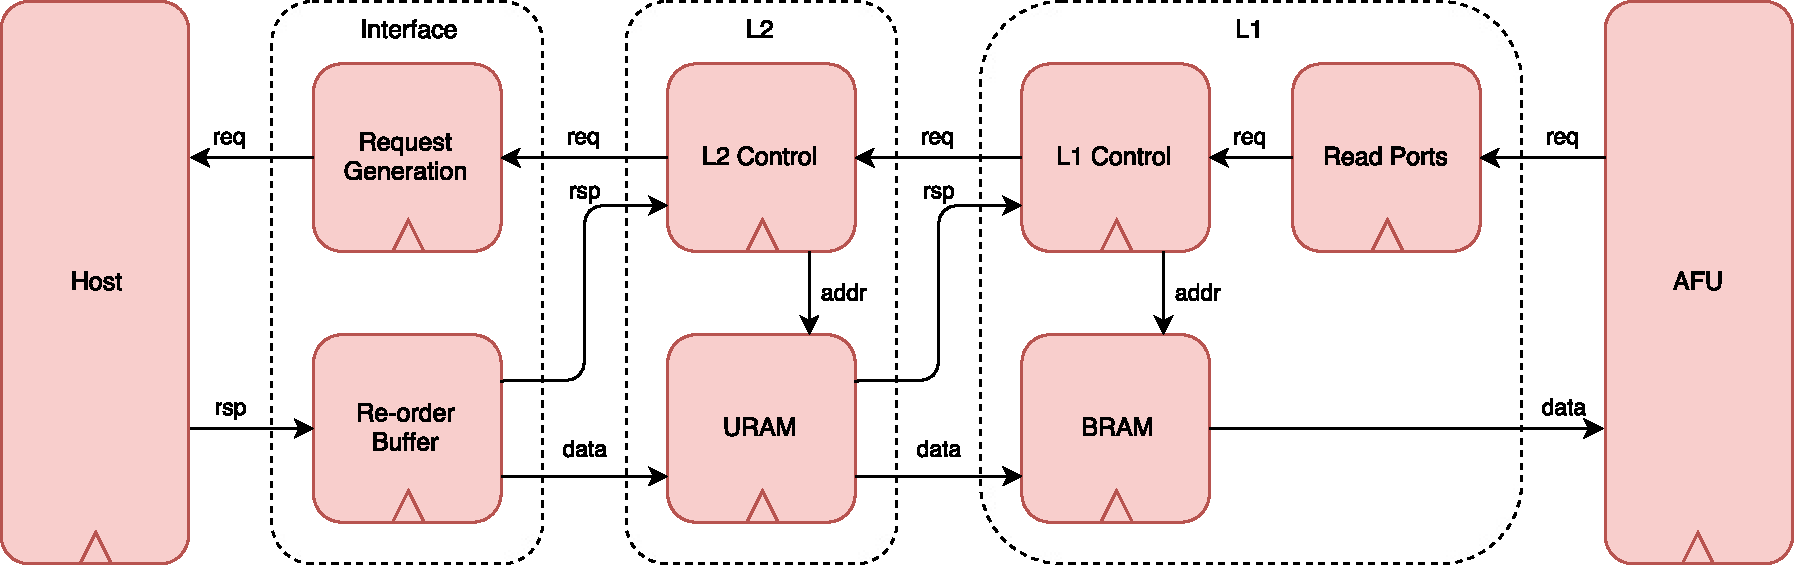
\includegraphics[width=0.95\textwidth]{7-apl-top.pdf}
  \caption{Diagram of the multi-stream buffer architecture.}
  \label{fig:7-apl-top}
\end{figure}




\subsection{Host Data Response Operation}
The complexities of OpenCAPI, or any interconnect for that matter, could be abstracted away by using for example an OpenCAPI-to-AXI bridge. A similar bridge exists for CAPI 1.0 as mentioned in Section \ref{sec:capi-1.0}. Attaching an AXI interface to the multi-stream buffer would make it portable across interconnect standards, especially since AXI is the de facto standard in the world of FGPAs.\\
Independent of the chosen interconnect to the host, interconnect standards often allow response to be transferred out-of-order. Since the multi-stream buffer architecture expects response to come back in-order, a \textit{Re-order Buffer} module is required. This module allows new cache lines to be written immediately to the \textit{URAM} module, but only sends a response to the respective \textit{L2 Control} module, which in turn updates the valid counter for that L2 stream pointer, if it is a consecutive response. If not, the response will be delayed until all previous response have been received.\\
When an L1 stream controller requests a new cache line from L2, the cache line is written simultaneously from the respective L2 buffer to all eight corresponding L1 stream buffers. Each individual connection between the \textit{URAM} and \textit{BRAM} module for such write operations is called a \textit{write channel}. Ideally each stream has its own write channel, but that results in a complex wiring job since each write channel has a width of 128 bytes or 1024 bits (wires). Each of the modules shown in \autoref{fig:7-apl-top} will be discussed in more detail in the remainder of this chapter.



\subsection{Functional Stream Reset Operation}
Before read requests from the AFU are accepted by the \textit{L1 Control} modules, the desired stream has to be functionally reset. A functional reset request consists of a ready-valid signal pair, a stream identifier and two addresses to indicate the start and end location of the data in host memory. This allows streams to consist of a different number of cache lines per stream. Both addresses have to be cache line size aligned, which is 128 bytes in this case.\\
The functional reset interface is not shown in \autoref{fig:7-apl-top} but is connected through a demultiplexer to each \textit{L2 Control} module. From there, each L2 controller is connected to the respective \textit{L1 Control} module which presents a one-hot signal to the AFU indicating whether a stream has finished or not. This signal is accompanied by a ready-valid signal pair such that the AFU can be notified when a functional reset has been accepted by both levels of stream controllers. The functional reset interface input could for example be connected to a sideband signal of the interconnect or an MMIO region on the FPGA card.\\
If a functional reset request is accepted, the respective \textit{L2 Control} module will start requesting cache lines from the host until its URAM is full. While requesting cache lines, the functional reset request is forwarded to the respective \textit{L1 Control} module. If the request is accepted, the module will start requesting cache lines from L2 until its BRAM is full. A reason for not accepting a functional reset request is for example when the stream has not yet finished its current stream and thus still holds valid data which is not allowed to be overwritten.\\
When the AFU sends a read request for a stream, it is only accepted if the stream has been reset and if at least two valid cache lines are present in the BRAM, since in the desired configuration the AFU is capable of reading across a cache line boundary. Corner cases exist which will be discussed in more detail in Section \ref{sec:deadlocks}.\\
While the interface modules have been briefly discussed from a functional perspective, the modules are not implemented in the final design. The \textit{Request Generation} module has been built and tested, but was not integrated within the verification framework discussed in Section \ref{sec:verif}. The module can be found on the GitHub page of this project \cite{yvo-lib}. Integrating both modules is left as future work.





\section{Multi-Stream Buffer Architecture Design Choices}
\label{sec:design-choice}
This section motivates the design choices made before the implementation phase. The most important choice to be made is determining the size of each level of buffering, while making sure the memory primitives are fully utilized. Due to the wide data paths, routing delay has to be taken into account.



\subsection{Buffer Depth Analysis}
\label{sec:buffer-depth}
For any configured number of read ports \textit{P}, at most \textit{P} new cache lines are requested from L2 during a single cycle. Ideally these requests are processed and written to the corresponding L1 buffer in parallel. Since all stream controllers in both levels operate in parallel, transmitting new cache line requests from L1 to L2 occurs in parallel as well. The system architecture shown in \autoref{fig:7-apl-top} suggests a single write channel between the L2 and L1 buffer. This could potentially become a point of congestion, depending on the AFU access pattern and the number of read ports, and result in an empty L1 buffer. An equal number of write channels as read ports is desired between L2 and L1 to minimize congestion. Each read port still has access to all streams, because the L1 buffers are duplicates of each other.\\
\autoref{fig:7-channels} shows a generalized diagram of the memory organization for multiple write channels. Each write channel services a fixed subset of streams, even though not fixing this would be better. However, such a solution requires each write channel to be able to access every stream. This is very expensive in terms of wiring since each write channel is 1024 bits wide and drives multiple BRAM slices. A BRAM or URAM slice is an array of possibly multiple memory primitives that share the same write interface. In principle, a slice could contain any number of streams. However, both the BRAM and URAM slice serve the same number of streams, be it with a different number of cache lines. In the case of the BRAM slice, the write channel drives as many BRAM arrays as there are read ports configured. This means that all BRAM slices with the same slice number are driven by the same URAM slice. In the figure this is shown by placing the BRAM slices horizontally next to each other. When multiple L2 requests for the same slice occur in the same cycle, the different requests are serviced in parallel by the corresponding stream controllers and merged using an arbiter for example before accessing the URAM slice, since only one read and one write interface is available per slice.

\begin{figure}[h]
  \centering
  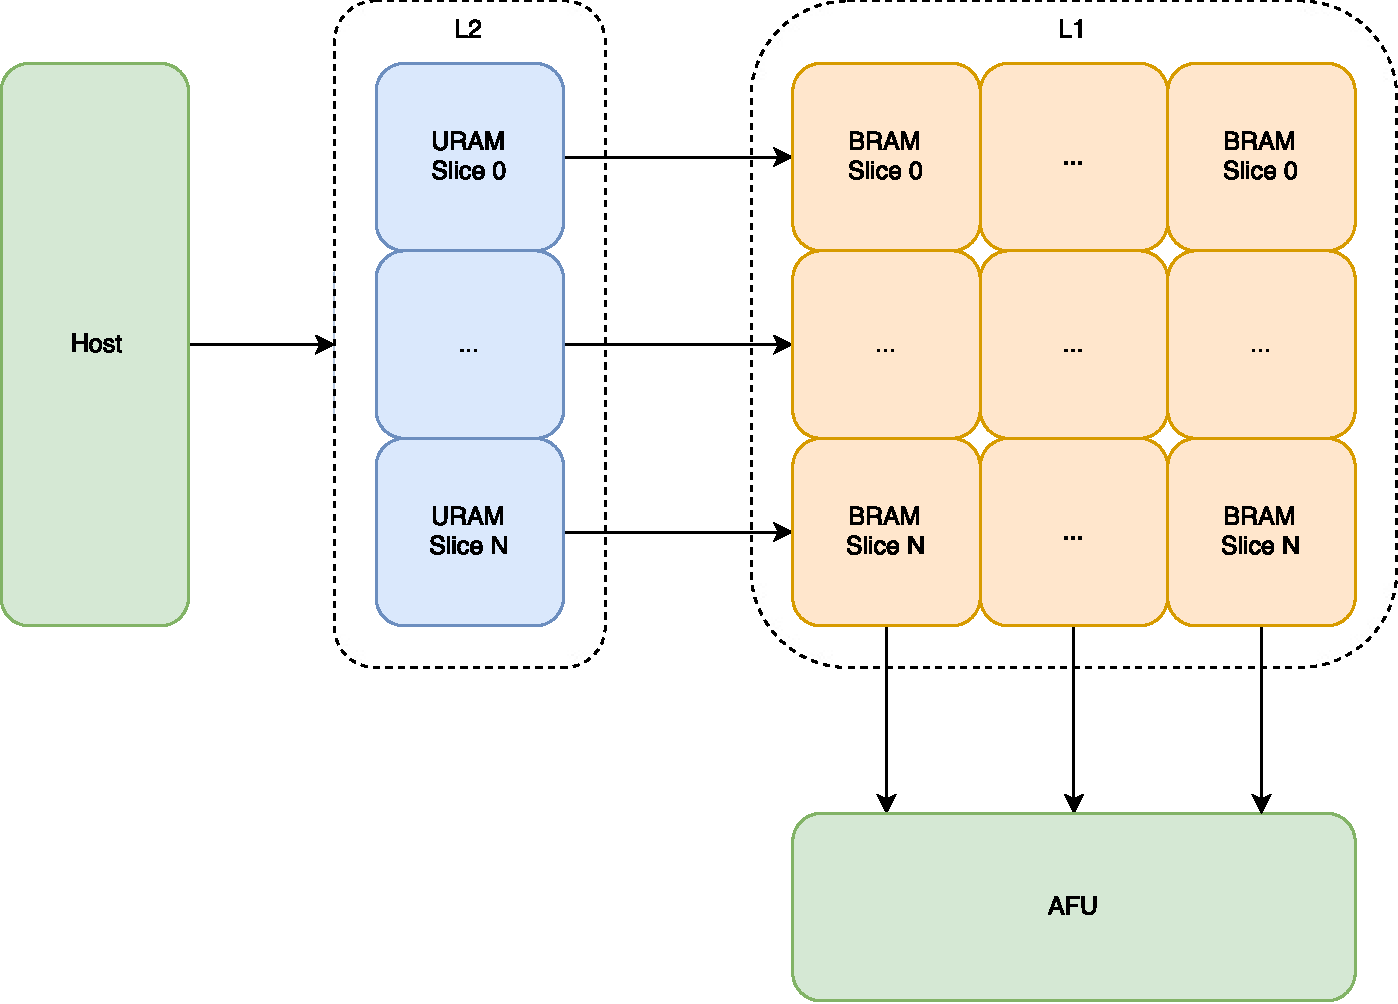
\includegraphics[width=0.70\textwidth]{7-channels.pdf}
  \caption{Diagram of the memory organization for multiple write channels.}
  \label{fig:7-channels}
\end{figure}



\subsubsection{AFU Access Patterns}
For any number of read ports, there are two distinct access patterns that both generate the maximum number of new cache line requests from L1 to L2 in one cycle. \autoref{fig:5-port-pattern} shows the requested stream per read port per cycle. This is under the assumption that each cache line consists of as many data elements as there are read ports. Another assumption is that each stream is read by starting from the first data element at offset zero. All read ports have a predefined priority, with port zero having the highest. That means that if multiple read ports request the same stream, the highest priority read port will return the first unread data element.\\
\autoref{fig:5-port-pattern-1} shows one case where all read ports read from the same stream in each cycle, for example stream zero. When the last element of a cache line is read, a request from L1 to L2 is made. In this case, this happens once every cycle as illustrated by the green box. After \textit{P} cycles of this pattern, \textit{P} cache lines have been requested, but the requests are evenly distributed as one per cycle. In this example \textit{P} equals eight.\\
\autoref{fig:5-port-pattern-2} shows the other case where all read ports read from different streams in a single cycle. For example, stream zero through \textit{P-1}. If such a pattern is sustained for \textit{P} cycles, also \textit{P} requests are made from L1 to L2 but all in the same cycle, which results in a burst of L2 requests. In this example \textit{P} equals eight.

\begin{figure}[h]
  \centering
  \begin{subfigure}[c]{.5\textwidth}
    \centering
    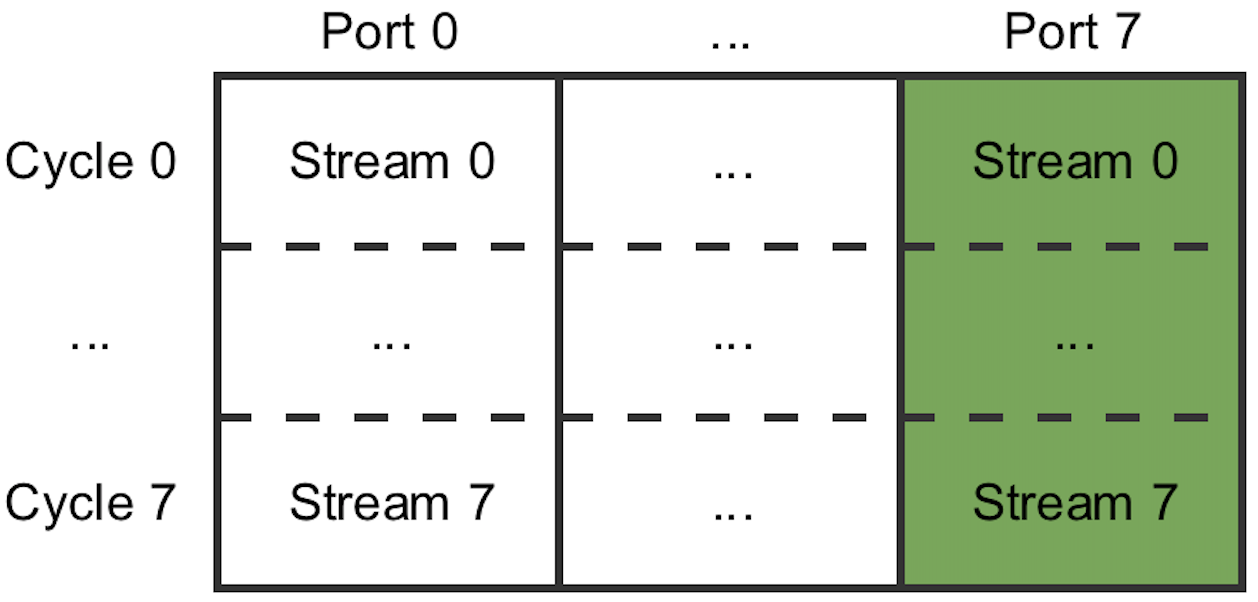
\includegraphics[width=0.8\linewidth]{5-port-pattern-1.png}
    \caption{Distributed L2 requests.}
    \label{fig:5-port-pattern-1}
  \end{subfigure}%
  \begin{subfigure}[c]{.5\textwidth}
    \centering
    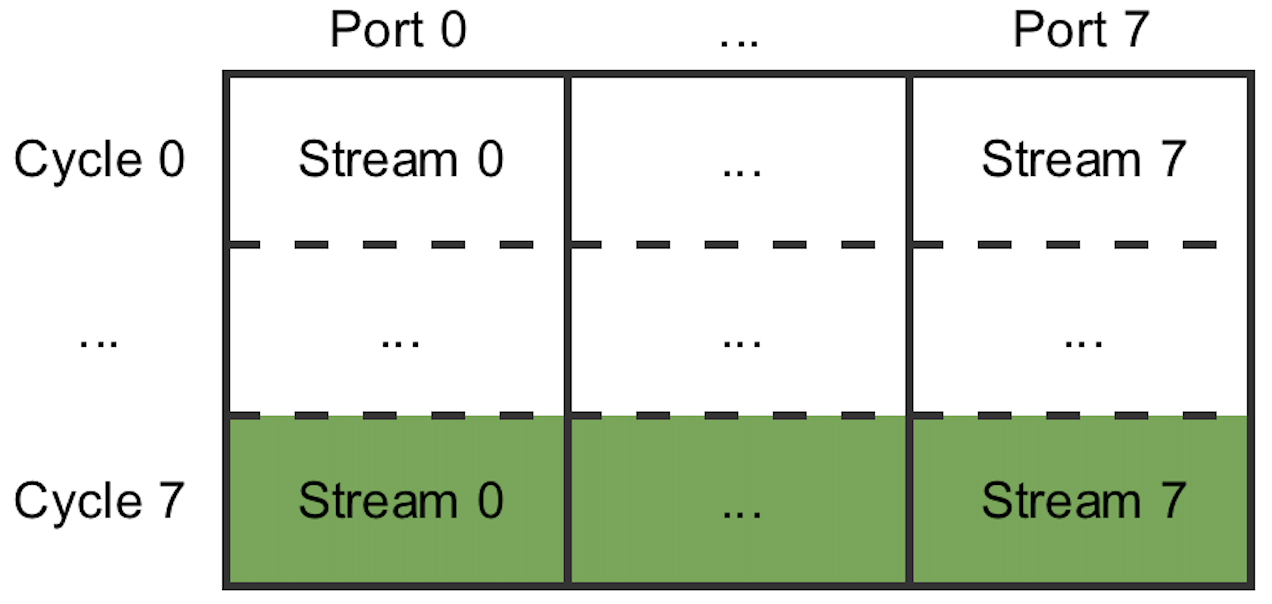
\includegraphics[width=0.8\linewidth]{5-port-pattern-2.png}
    \caption{Burst of L2 requests.}
    \label{fig:5-port-pattern-2}
  \end{subfigure}
  \caption{Eight read port stream access pattern.}
  \label{fig:5-port-pattern}
\end{figure}

%In the worst case, the AFU starts reading from eight different streams from the same slice in cycle \textit{N}, as shown in \autoref{fig:5-port-pattern-2}. This results in a burst of L2 requests and eight new cache lines have to be written from L2 to L1. Since there is only one write channel per bank, this will take eight cycles to complete. If in cycle \textit{N+1} a full cache line is read from one of the eight streams requested in cycle \textit{N}, as shown in \autoref{fig:5-port-pattern-1}, again a new cache line is requested for that stream. Assume that writing a new cache line from L2 takes one cycle and that the requested cache lines are available in L2. This new L2 request will be serviced by the stream controller in parallel with the others. However, it will be queued up behind the other seven outstanding requests from cycle \textit{N}, since every new cache line will have to be written using the same write channel.



\subsubsection{Stream Exhaustion}
When the burst access pattern is succeeded by the distributed access pattern and both request streams from the same slice, L2 requests made by the distributed access pattern are queued up behind those of the burst access pattern. This is under the assumption that L2 requests are queued in ascending order, starting with stream zero. Depending on various factors such as the number of streams per slice, the latency of the control logic and memory organization, and the number of read ports, an L1 stream buffer could get exhausted. This is undesired behaviour and the L1 buffer should be adequately large.\\
\autoref{fig:5-access-pattern} illustrates a generalization of this worst case scenario by combining both access patterns. \autoref{fig:5-access-pattern-1} shows a configuration with \textit{P} read ports. The access pattern shown is preceded by AFU read requests which resulted in a state where each stream has only one unread data element left in the current cache line. Therefore, when a stream is read, an L2 request is made.\\
For a configuration with a total number of streams \textit{N} and \textit{C} write channels, each slice services $\frac{N}{C}$ streams. To obtain a queue of L2 requests, the burst pattern is triggered using all read ports for $\frac{N}{C \times P}$ consecutive cycles to trigger all streams within this slice. The green boxes indicate a burst pattern read request resulting in an L2 request.\\
Next, stream $\frac{N}{C}-1$ is read, the stream with the highest number, using the distributed access pattern. Under the assumption that streams are serviced in ascending order means that the highest numbered stream is in the last batch of read requests. If only this stream is read from here on, it will have to survive the longest number of cycles before a new cache line will be written into the corresponding L1 buffer, since the request is queued up behind requests from all other streams. The orange boxes indicate a distributed pattern read request, that could result in an L2 request. This depends on rate \textit{R} and will be discussed later.

\begin{figure}[h]
  \centering
  \begin{subfigure}[c]{.35\textwidth}
    \centering
    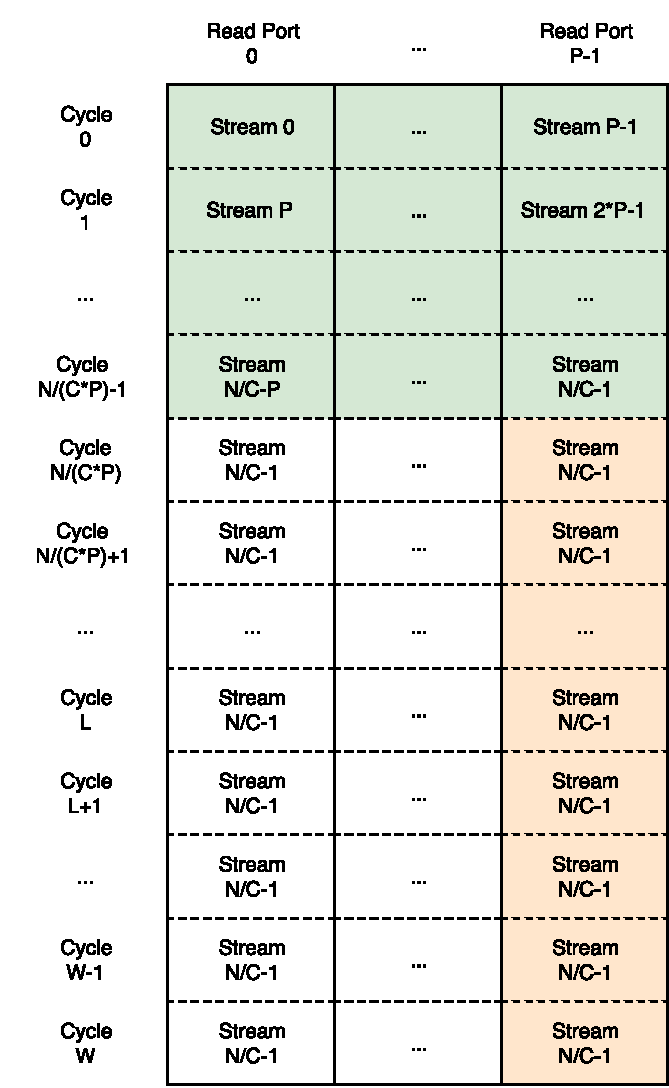
\includegraphics[width=0.95\linewidth]{5-access-pattern-1.pdf}
    \caption{Requested stream per read port.}
    \label{fig:5-access-pattern-1}
  \end{subfigure}%
  \begin{subfigure}[c]{.65\textwidth}
    \centering
    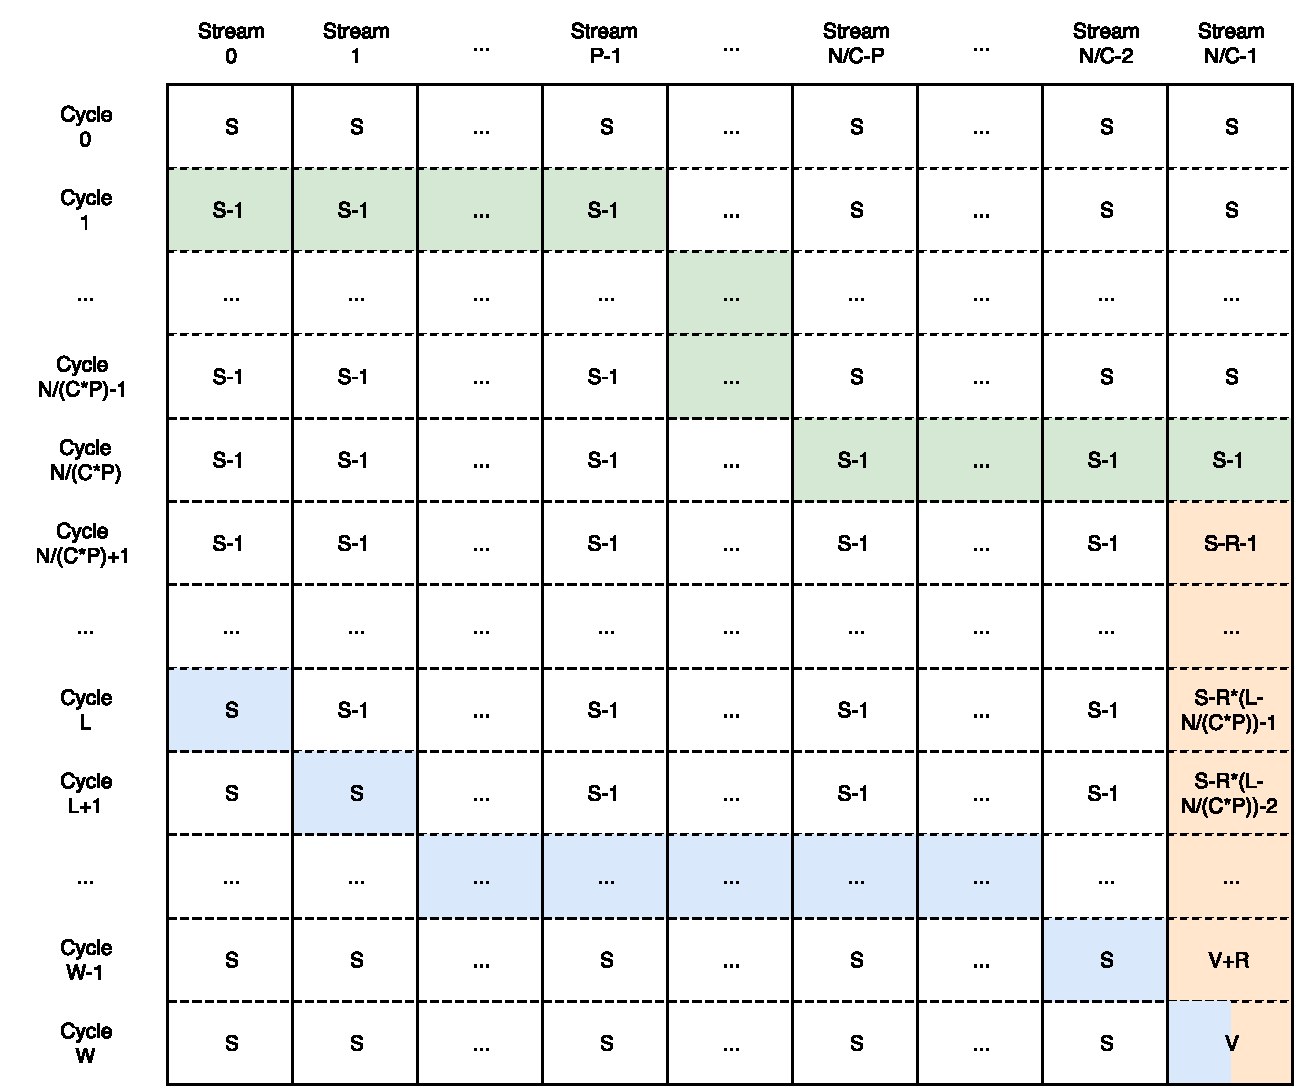
\includegraphics[width=1.00\linewidth]{5-access-pattern-2.pdf}
    \caption{Number of valid cache lines present per stream.}
    \label{fig:5-access-pattern-2}
  \end{subfigure}
  \caption{Generalized worst case AFU access pattern.}
  \label{fig:5-access-pattern}
\end{figure}

\autoref{fig:5-access-pattern-2} shows for each stream the number of valid cache lines present, as a result of the read access pattern shown in \autoref{fig:5-access-pattern-1}. In the initial state in cycle zero, each buffer is full with \textit{S} valid cache lines. The valid counters per stream reflect changes due to the AFU access pattern in the consecutive cycle the AFU read request was made. As an example, in cycle one the green boxes indicate a change in the number of valid cache lines for the first \textit{P} streams due to the burst pattern triggered in cycle zero in \autoref{fig:5-access-pattern-1}. The burst pattern continues until cycle $\frac{N}{C \times P}$.\\
Rate \textit{R} is defined as $\frac{P}{E}$ and indicates how many cache lines can be requested per cycle for the distributed pattern. During the burst pattern it is known that a cache line from L2 will be requested. Therefore the valid counters are decreased by one. For subsequent cycles, this depends on the chosen configuration of the number of data elements per cache line \textit{E} and the number of read ports \textit{P}. This is under the assumption that \textit{P} is always smaller or equal than \textit{E}.\\
Cycle \textit{L} indicates when the first L2 request has been completed and a new cache line has been written in the corresponding BRAM array depends on the latency of the stream controllers and the memory primitives. Cycle \textit{L} is defined as the sum of the \textit{L2 Control}, \textit{URAM}, and \textit{BRAM} module latencies. Or in other words, the latency between issuing an L2 request and writing the corresponding cache line into the BRAM array. From cycle \textit{L} onward, blue boxes indicate that a new cache line has been written and therefore the valid counter has increased by one. Since each BRAM slice has only one write interface, there is an imbalance between the generation and servicing of an L2 request by a factor of \textit{P} to one. That means that in a single cycle, at most \textit{P} L2 requests can be issued, while at best only one new cache line can be written.\\
At cycle \textit{W}, the initial L2 request made by stream $\frac{N}{C}-1$ has been written into the corresponding BRAM array. In essence, stream $\frac{N}{C}-1$ has to survive until cycle \textit{W} and equals $\frac{N}{C}+L-1$. To calculate the buffer size \textit{S}, an additional constraint \textit{V} is added that indicates the minimum number of valid cache lines required to accept an AFU read request.

%\subsubsection{OLD}
%\autoref{fig:5-access-pattern} visualizes a generalization of this access pattern, where the number of buffered cache lines per stream \textit{S} covers the latency \textit{L} and the outstanding L2 requests $O_{max}$. It should be noted that for certain configurations, actions might overlap and occur in the same cycle. For example, reading in the burst access pattern and writing a new cache line into L1. Both sub-figures are annotated with variables which are explained in \autoref{eq:omax}. \autoref{fig:5-access-pattern-1} shows the stream requested for each read port by the AFU. A green box indicates that the respective read request results in an L2 request. \autoref{fig:5-access-pattern-2} shows how many valid cache lines are present in each stream within one bank. Assume that an L1 buffer can only be read after a functional reset, when it is completely filled with valid cache lines. One or multiple L2 requests, resulting from reading a cache line completely, are reflected in the next cycle in \autoref{fig:5-access-pattern-2}, indicated by a green box for that particular stream.\\
%Depending on the number of streams per bank, the burst access pattern occurs for $\frac{N}{C \times P}$ cycles. In the next cycle, the other access pattern is initiated. Assume that new cache lines are written from L2 in order of increasing stream number, starting at stream zero. In that case, stream $\frac{N}{C}-1$ will be updated last. This stream will be called the target stream from now on. Due to this AFU access pattern, the target stream will be drained first, something that is not desired since it limits throughput. After a certain latency \textit{L}, the first L2 request has been serviced, indicated by the blue box. The write operation into stream zero started a cycle earlier, due to the single write latency of BRAM. Every cycle, a new cache line is written in L1, while the target stream is drained slowly. In cycle \textit{S}, both a cache line is read and a new one is written in the target stream, resulting in an equilibrium indicated by both a green and blue box. As mentioned before, this is a perfect example where the number of buffered cache lines \textit{S} covers the worst case AFU access pattern.\\

%In accordance with the generalized worst case AFU access pattern, the maximum number of outstanding L2 requests $O {max}$ per bank with one write channel can be computed as follows.
%\begin{itemize}
%  \item{$O {max}$ is the maximum number of outstanding L2 requests.}
%  \item{\textit{N} is the total number of streams.}
%  \item{\textit{P} is the total number of AFU read ports.}
%  \item{\textit{L} is the latency from making the first L2 request to the first cache line written in the L1 buffer. This is the sum of the L1 and L2 control logic latency, the URAM read latency and the one cycle latency of writing BRAM.}
%  \item{\textit{C} is the number of write channels between L2 and L1.}
%\end{itemize}

%\begin{equation}
  %O {max} = N + L - \frac{N}{R} - 1
%  O {max} = \frac{N}{C} - \frac{N}{C \times P} + L - 1
%  \label{eq:omax}
%\end{equation}

%The maximum number of outstanding L2 requests is roughly equal to the total number of streams \textit{N}. If there are more streams than read ports, there are multiple consecutive cycles of the access pattern shown in \autoref{fig:5-port-pattern-2}. This results in a queue of L2 requests due to the limited number of write channels. Each cycle this happens, an L2 request has advanced and a new cache line can be written. Therefore the number of cycles this happens is subtracted. When all \textit{N} streams have triggered an L2 request, the AFU will read according to the access pattern shown in \autoref{fig:5-port-pattern-1}. This results in an additional L2 request every cycle targeting stream \textit{N - 1} in order to drain its L1 buffer. Additionally, the latency \textit{L} has to be covered and the larger \textit{L}, the more targeted L2 requests can be made before reaching an equilibrium of reading and writing the L1 buffer. The actual number of streams per bank is obtained by dividing the total number of streams \textit{N} by the number of write channels \textit{C}. Finally, one is subtracted because at least one valid cache line has to be present in the L1 buffer in order to not read and write at the same address. This address collision results in a stall because SDP BRAM primitives allow only for reading and writing to the same address in a read-before-write fashion, as mentioned in Section \ref{sec:fpga-characterization}. Due to the nature of streaming, both the read and write addresses per stream are always consecutive, known a priori, and wrap-around at the last address.\\
%As an example, assume a configuration where $\frac{N}{C}$ is eight, \textit{S} is sixteen and reading the targeted stream starts at address zero. First, the AFU reads according to the burst access pattern. The other, in this case fifteen, cache lines in L1 for this stream are read according to the distributed AFU access pattern, one cache line per cycle. The first new cache line to be written, originating from L2, is written at address zero since that is the cache line which was read first. If writing the new cache line occurs during the same cycle as reading the next cache line, which wrapped-around and is at address zero again, there is an address collision in the BRAM primitive. Therefore the first new line written in L1 for the targeted stream has to be written at least one cycle before it is read.

%In the interleaved architecture with eight write channels, each bank can have a maximum number of outstanding L2 requests of $6 + L$, or seven as mentioned before if latency \textit{L} is assumed to be one. If each write channel would be able to operate with any bank, complex scheduling logic is required which increases latency, while latency should be minimized. It seems that implementing such a scheme will only benefit this rare case, while the common case should be made faster. Therefore, each write channel is limited to a single bank, basically resulting in the initial proposed architecture from Section \ref{sec:design-choice}, but then parallelized by banking multiple streams and having every stream controller in both levels operate independently.



\subsubsection{L1 Buffer Depth}
\label{sec:buffer}
To determine the L1 buffer size per stream \textit{S}, \autoref{fig:5-access-pattern} and the associated access pattern is analyzed. Due to the initial burst pattern, at least one cache line has to be buffered. This is the cache line consumed within the first $\frac{N}{C \times P}$ cycles for every stream. In order to survive until cycle \textit{W}, a minimum number of valid cache lines \textit{V} must be present in the buffer. In between these two events, stream $\frac{N}{C}-1$ is read according to the distributed pattern and makes L2 requests at rate \textit{R}. The number of cycles between the two earlier mentioned events is multiplied by rate \textit{R} to obtain Equation \ref{eq:s}.

\begin{equation}
  S = R \times \bigg( W - \frac{N}{C \times P} \bigg) + V + 1 \implies \frac{P}{E} \times \bigg( \frac{N}{C} + L - 1 - \frac{N}{C \times P} \bigg) + V + 1, \text{where}
  \label{eq:s}
\end{equation}

\begin{itemize}
  \item{\textit{S} is the number of cache lines to buffer per stream,}
  \item{\textit{R} is the rate at which L2 requests are issued during the distributed access pattern,}
  \item{\textit{W} is the cycle in which the initially requested cache line by stream $\frac{N}{C}-1$ is written into the BRAM array,}
  \item{\textit{N} is the total number of streams,}
  \item{\textit{C} is the number of write channels,}
  \item{\textit{P} is the number of read ports,}
  \item{\textit{V} is the minimum number of valid cache lines present in the BRAM array in order to service an AFU read request,}
  \item{\textit{L} is the sum of the \textit{L2 Control}, \textit{URAM}, and \textit{BRAM} module latencies, and}
  \item{\textit{E} is the number of data elements within a cache line.}
\end{itemize}



Equation \ref{eq:s2} shows the buffer size \textit{S} when using the requirements for the multi-stream buffer as mentioned in Section \ref{sec:reqs}. \textit{V} equals two such that the AFU is always able to read across a cache line boundary. Only servicing a read request when there are two or more valid cache lines makes complex logic, for when only one valid cache line is present, unnecessary.

\begin{equation}
  S = \frac{64}{C} + L - \frac{64}{C \times 8} + 2
  \label{eq:s2}
\end{equation}

Since the number of write channels \textit{C} is limited, a series of approximations of the buffer size can be made. \autoref{tab:est} shows the number of write channels versus the buffer size per stream. The benefit of multiple write channels is obvious, but the cost of a write channel in terms of routing complexity has to be taken into account.

\begin{table}[H]
  \centering
  \caption{Buffer sizes for a variety of write channels.}
  \label{tab:est}
  \begin{tabular}{ c | c }
    \textbf{C} & \textbf{S} \\ \hline
    1 & \textit{L + 58} \\
    2 & \textit{L + 30} \\
    4 & \textit{L + 16} \\
    8 & \textit{L + 9} \\
  \end{tabular}
\end{table}

Based on this analysis, multiple configurations are possible, depending on the AFU access pattern, target FPGA, the latency of control logic and memory arrays, and many more. In the following sections the BRAM primitive configurations and routing complexity will be taken into account in order to make a final decision on the number of write channels.

%Variations are possible, where for example if \textit{L} is increased, more cache lines should be buffered. Otherwise the target stream will become entirely drained. Changing the number of streams per bank for example influences the start of the second access pattern, but also increases the latency of writing the initially requested cache line from L2 into L1.

%In order to determine the depth of each L1 stream, or the number of cache lines to buffer \textit{S}, several other factors have to be taken into account. Besides $O {max}$, including latency \textit{L}, there is the initial cache line that was read in cycle \textit{N}. Also, an additional entry is required because while the expression for $O {max}$ in \autoref{eq:omax} subtracts one entry due to the nature of SDP BRAM primitives, a cache line has to be buffered during that cycle. The following equation summarizes this analysis starting from the moment the L1 control logic receives a request from the read port logic. \textit{L} has been replaced with the summation of the respective logic latencies. The earlier assumption of a latency \textit{L} of one seems unrealistic since a URAM primitive alone has a one to four cycle access time, depending on the target frequency. Also, additional latency has to be taken into account for the respective control logic.

%\begin{itemize}
%  \item{\textit{S} is the number of cache lines to buffer per stream.}
%  \item{\textit{R} is the cache line read in cycle \textit{N}, therefore equal to one.}
%  \item{$O {max}$ is the maximum number of L2 requests behind which a new request made in cycle \textit{N+1} can be queued up.}
%  \item{$L 1$ is the latency of the L1 control logic.}
%  \item{$L 2$ is the latency of the L2 control logic.}
%  \item{\textit{U} is the maximum latency when reading a URAM memory primitive.}
%  \item{\textit{B} is the one cycle latency of writing a BRAM memory primitive.}
%\end{itemize}

%\begin{equation}
%  S = R + O {max} + 1 = R + \frac{N}{C} - \frac{N}{C \times P} + L 1 + L 2 + U + B
  %\implies 1 + 6 + L 1 + L 2 + 4 + 1 + 1 = L 1 + L 2 + 13
%  \label{eq:s}
%\end{equation}

%Plugging numbers into \autoref{eq:s} according to the eight write channel configuration and the worst case for the memory accesses, \textit{S} equals $13 + L 1 + L 2$. Buffering sixteen cache lines per stream (the next power of two) results in a maximum latency of three cycles for the control logic. While this may seem to be too little, bear in mind that this AFU access pattern is very specific and seems quite unlikely to occur. However, if the target AFU does have such an access pattern, this parameter can be configured accordingly due to the nature of FPGAs.



\subsubsection{L2 Buffer Depth}
\label{sec:l2-buffer-depth}
Determining the number of cache lines per stream to buffer for L2 is less complex compared to L1. The goal of the L2 buffer is to hide the latency of OpenCAPI. At best, one cache line is received per cycle from the host through OpenCAPI.\\
No real-world latency numbers are published for OpenCAPI at the moment of writing. Since one of the goals of OpenCAPI is to deliver a lower latency than current interconnect standards, a typical latency of PCI Express Gen 3 of \SI{1}{\micro\second} is used as a conservative upper bound as mentioned in \ref{sec:pciegen3}. Assuming that the FPGA operates at \SI{200}{\mega\hertz}, 200 cycles on the FPGA have to be covered and thus 200 cache lines have to be buffered. An access pattern where only one stream is constantly requested could occur. Rounding this up to the next power of two results in 256 cycles, or cache lines, to buffer per stream.



%\todo



\subsection{BRAM Sharing Among Streams}
\label{sec:sharing}
Section \ref{sec:buffer-depth} made the assumption that the underlying BRAM primitives were utilized perfectly. While this is fine for a first-order analysis, the BRAM primitive configuration has to be taken into account during implementation. For example, implementing a single stream per BRAM primitive is very wasteful because only sixteen entries are used per BRAM which equals to a utilization of roughly 3\%. Double pumping makes no significant difference. Therefore, BRAM primitives have to be shared among streams in order to achieve full utilization. Without double pumping, a BRAM primitive is fully utilized with 32 streams and with double pumping 16 streams are required. For example, in a configuration with eight write channels, or eight streams per slice, each BRAM primitive is only utilized for 50\%. A deeper analysis has to be made in order to find the optimal number of write channels.

%\todo{- for certain BRAM configs, mention the total BRAM primitive utilization as well, to compare to naive designs.\\}



\subsection{Multiple Write Channels Analysis}
%If a single write channel is used for all streams, the maximum number of outstanding L2 requests increase dramatically.

%If this is generalized across all 64 streams, it becomes clear that the number of outstanding L2 requests increase dramatically. Since there is only one write channel between L2 and L1, there are scenarios possible where congestion occurs due to the bottleneck of having only one write channel.

%To illustrate this, the maximum number of outstanding L2 requests can be computed as follows, under the assumptions that there is only one write channel present and that the requested cache line in L2 is available.
%\begin{itemize}
%  \item{$O {max}$ is the maximum number of outstanding L2 requests.}
%  \item{\textit{N} is the total number of streams.}
%  \item{\textit{R} is the total number of AFU read ports.}
%  \item{\textit{L} is the latency from making the first L2 request to the first cache line written in the L1 buffer. Expressed in previously mentioned terms, this is the sum of the L1 and L2 control logic, the URAM read latency and the one cycle latency of writing BRAM.}
%\end{itemize}
%\begin{equation}
%  O {max} = N + L - \frac{N}{R} - 1
%  \label{eq:omax}
%\end{equation}
%The maximum number of outstanding L2 requests is roughly equal to the total number of streams \textit{N}. If there are more streams than read ports, there are multiple consecutive cycles of the access pattern shown in \autoref{fig:5-port-pattern-2}. This results in a queue of L2 requests due to the limited number of write channels. Each cycle this happens, an L2 request has advanced a cycle and a new cache line can be written. Therefore the number of cycles this happens is subtracted. When all \textit{N} streams have triggered an L2 request, the AFU will read according to the access pattern shown in \autoref{fig:5-port-pattern-1}. This results in an additional L2 request every cycle targeting stream \textit{N - 1} in order to drain its L1 buffer. Additionally, the latency \textit{L} has to be covered and the larger \textit{L}, the more targeted L2 requests can be made before reaching an equilibrium of reading and writing the L1 buffer. Finally, one is subtracted because at least one valid cache line has to be present in the L1 buffer in order to not have an address collision, which results in a stall. This is due to the fact that SDP BRAM primitives do allow for reading and writing to the same address, but only in a read-before-write fashion, as mentioned in Section \ref{sec:fpga-characterization}. Due to the nature of streaming, both the read and write addresses per stream are always consecutive, therefore known a priori, and wrap-around at the last address.\\
%As an example, assume that reading the targeted stream starts at address zero. This occurs using the initial AFU access pattern. The other, in this case fifteen, cache lines in L1 for this stream are read according to the second AFU access pattern, one cache line per cycle. The first new cache line to be written, originating from L2, is written at address zero since that is the cache line which was read first. If the writing the new cache line occurs during the same cycle as reading the next cache line, which wrapped-around and is at address zero again, there is an address collision in the BRAM primitive. Therefore the first new line written in L1 for the targeted stream has to be written at least one cycle before it is read.

Section \ref{sec:buffer-depth} showed that for a specific AFU access pattern outstanding L2 requests get queued up and a specific L1 stream buffer could become exhausted. Under the worst case memory access assumption and a configuration of 64 streams and one write channel, the required L1 buffer should contain at least 64 cache lines. It is obvious that with this architecture, the L1 buffer can get exhausted, resulting in stalls and degradation of throughput. The congestion of L2 requests can be improved by increasing the number of write channels between L2 and L1, such that potentially multiple new cache lines can be written in L1. Multiple write channels delay and might even prevent the exhausted state of the L1 buffer, depending on the number of write channels and the latency of surrounding logic and memory arrays. There is an incentive to minimize latency \textit{L} because it enables to delay total exhaustion of the target L1 stream buffer. Since each L2 stream buffer ideally contains 256 cache lines, there should be more than enough cache lines ready to be written into the L1 buffer. The number of write channels is however bounded in two ways.

\begin{itemize}
  \item{\textbf{BRAM Utilization} impacts the number of streams per BRAM primitive and therefore the number of write channels which can be efficiently implemented. As shown in Section \ref{sec:sharing}, each primitive is fully utilized with 16 or 32 streams. By dividing the streams across several BRAM primitives, the streams are interleaved. This efficient number of streams per BRAM means that the only possible number of write channels, which results in an evenly distributed number of streams per slice, is either one, two or four. It is desired to distribute the number of streams evenly across write channels in order to have a balanced system. If BRAM primitives are under-utilized, the required number of BRAM primitives will explode and the design will not fit within the KU15P's resource budget.}
  \item{\textbf{Write Channel Wiring} impacts the resource budget of the KU15P. Each channel requires 1024 bits. With multiple write channels, this results in a wiring nightmare and difficulty to route the design. However, the more write channels, the smaller the maximum congestion per slice.}
\end{itemize}

Ideally, the system is balanced where each AFU read port is backed up by its own write channel as mentioned earlier. However, eight write channels result in an under-utilization of BRAM primitives, therefore an explosion of required primitives, and requires 8192 wires, making routing more complex. This leaves the two and four write channel designs. A big benefit of the four write channel design is that this results in using sixteen streams per BRAM primitive, double-pumped. Because of the double-pumping, the physical write channel can also be double-pumped which means that 512 wires are used instead of 1024. Therefore, without any significant changes in logic, the same number of wires are required for a two or four write channel design, while the four write channel design avoids congestion by roughly a factor of two, under the assumption that latency \textit{L} is equal for both, compared to the two write channel design.
%Using \autoref{eq:omax} and the same variables as before, the maximum outstanding L2 requests per slice are $27 + L$ and $13 + L$ respectively for each design. This is a significant improvement compared to the single write channel case of $55 + L$. For the two and four write channel designs, \textit{S} equals $34 + L 1 + L 2$ and $20 + L 1 + L 2$ respectively. While four channels do not guarantee that an L1 buffer becomes fully drained, it does protect against a fair share of the worst case AFU access pattern while not under-utilizing BRAM or URAM primitives. Therefore, in order to keep up with the OpenCAPI bandwidth and basically have a no-compromise design, the four write channel design is chosen.



\subsection{Buffer Memory Organization}
\autoref{fig:5-memory} shows the final memory organization for the multi-stream buffer architecture, based on the previous sections in this chapter. The control flow starts at the AFU, which is able to request eight new elements per cycle. Each read port has its own logic to distribute the request among the different stream controllers (not shown). Every stream has a separate controller per level, while the cache lines per stream share memory primitives. This is because the minimum number of entries per memory primitive is much larger than what is required per stream. Sharing memory primitives between streams is not a problem, since cache lines are duplicated in L1 and each read port has access to a consecutive subset of cache lines per stream. Each AFU read port will at most request one element per cycle and therefore no conflict can occur per read port. Since all stream controllers operate independently and are connected directly to each other per stream, multiple new cache line requests in L2 can be serviced per cycle. By keeping the stream controllers independent and merging L2 requests only at the very last moment, when accessing the URAM and writing it to L1, throughput can be sustained for as long as possible. The only point of congestion is each write channel per slice. New data between the two levels is written in cache line granularity since complex logic would be required to replace single elements per stream for example.

\begin{figure}[H]
  \centering
  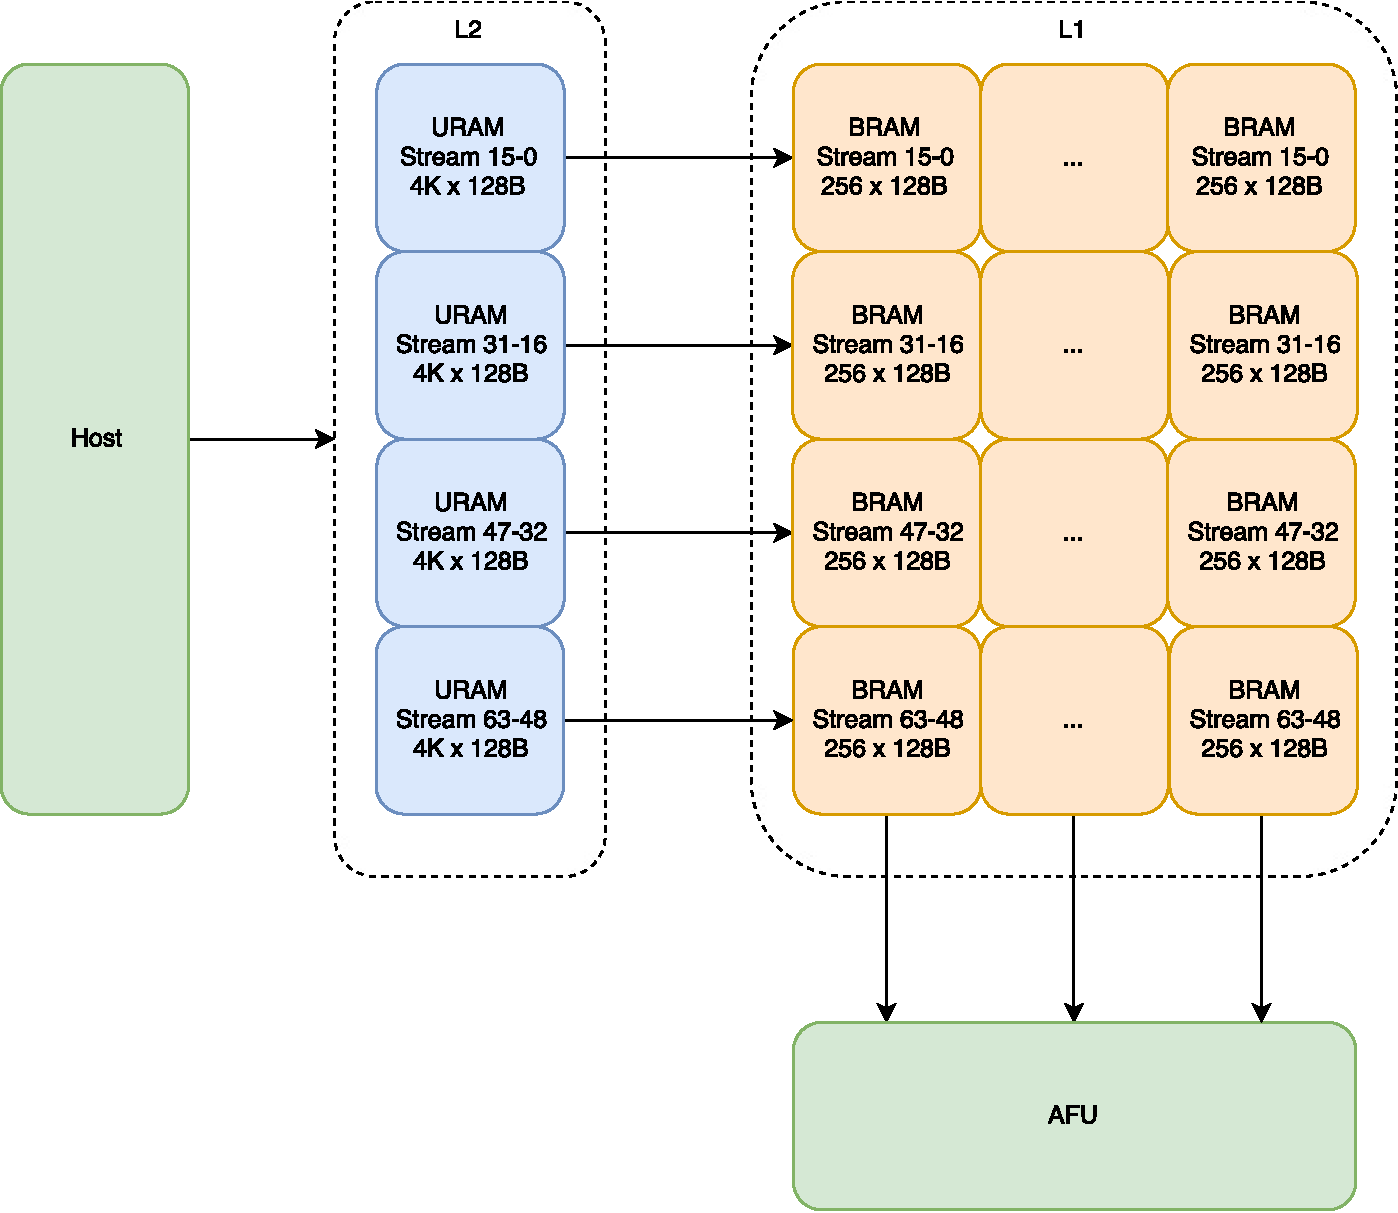
\includegraphics[width=0.65\textwidth]{7-channels-2.pdf}
  \caption{Memory organization of both buffer levels.}
  \label{fig:5-memory}
\end{figure}

\subsubsection{L2 Primitive Organization}
OpenCAPI can provide at most one \SI{128}{\byte} per \SI{200}{\mega\hertz} cycle. This cache line is then written in the corresponding URAM of the requested stream. Since there are four write channels, L2 is divided in four slices where each slice houses sixteen streams, each containing 256 cache lines. This results in 4096 entries. Since the memories are double pumped, two URAM primitives are required to obtain this number of entries. Cascading multiple \SI{8}{\byte} wide primitives results in a cache line-width buffer.

\subsubsection{L1 Primitive Organization}
Similarly, L1 also consists of four slices where each slice houses sixteen streams, consisting of sixteen cache lines per stream. This results in 256 entries. However, all of these cache lines are replicated for each read port to solve the multi-read-port problem. When a new cache line is written from L2 to L1, that data is written simultaneously to all eight corresponding slices. By double pumping the BRAM primitive in a 512 entry \SI{8}{\byte} wide configuration, a single BRAM primitive supplies all required entries at data element width. Then multiple primitives can be cascaded in order to obtain a cache line wide buffer.\\
For both levels the cache lines are direct mapped. During the functional reset of a stream, a start and end address are provided from which cache lines are automatically fetched. Based on the stream number and the physical address of a cache line, the address within a memory primitive is calculated. By direct mapping cache lines, the architecture might be extended in the future to act as a cache.





\subsection{Expected Resource Utilization}
The architecture described in this section has eight copies of sixteen cache lines per stream. In total, this will consume 256 BRAM primitives or 26\% of what is available for the desired configuration. Each stream buffers 256 cache lines in L2. This will consume 64 URAM primitives or 50\% of the total. Since sixteen streams share the same BRAM primitive, the multiplexing structure is smaller compared to the previous proposals. In this architecture, each read port selects the correct data element per slice, after which the correct slice is selected. This results in a 32:1 multiplexer at half the element width since the BRAMs are double-pumped. Roughly 2.6\% of the available LUTs are required.\\
The large improvement in LUT utilization is due to the fact that BRAM primitives are shared by multiple streams. Therefore the primitive takes care of a large part of the selection structure, especially at these data widths. Double-pumping also has a large impact. A careful reader might ask why this architecture was chosen, since a significant portion of both BRAM and URAM resources will be consumed. The element-wise double-pumped architecture might work just as fine. While this might be true at first sight, the proposed architecture considers the anticipated routing problems and takes the FPGA topology into account. The BRAMs are situated in a vertical direction on the FPGA, which makes guaranteeing the same read latency for every location very difficult. Placing a subset of cache lines a special, smaller, L1 ensures that less cache lines have to have the same low access latency and makes closing timing easier. Besides that, this architecture consumes the least number of BRAMs of all proposals. Therefore most primitives are left for use by the AFU (and DLX and TLX layers).

% brams = 8 brams per 16 streams * 4 write channels * 8 read ports = 256 brams / 984
% urams = 8 urams per 16 streams * 2 urams high * 4 write channels = 64 urams / 128
% luts = 32 to 1 mux = 9 * 64 bits wide = 192 * 8 read ports = 13824 luts / 522720





\subsection{Design Implementation Details}
Now that the high-level design choices have been motivated, each level of the design will be discussed separately, based on the modules presented in \autoref{fig:7-apl-top}. The whole design is based around a request-response philosophy, where requests are made between modules and responses are given back. Implicitly this is done by using the design methodology described in Chapter \ref{ch:method}. Explicitly this is done by, for example, viewing an AFU read as a request containing a stream identifier, which is followed by a response containing the same stream identifier and associated requested data. The entire project can be found on GitHub \cite{yvo-lib}.





\section{L1 Control}
The first level of the design, shown in \autoref{fig:5-l1-ctrl-top}, consists of the read port logic, L1 stream pointer logic and a transpose module. In the desired configuration, each of the eight read ports has its own read port module and BRAM array, while each of the 64 streams has its own pointer module, indicated by \textit{N} and \textit{M} respectively. Note that the arrows drawn only represent the valid and, if present, the associated data signal. The associated ready signal is most often not explicitly drawn.\\
The read port module calculates the address to index the respective BRAM array and requests new cache lines from L2 if necessary. Since each read port outputs the requested stream identifier as a decoded signal (one-hot), the input of the transpose module is a matrix with the number of read ports as entries, where each entry is the number of streams wide. Since each L1 stream pointer module is only interested in requests made for that particular stream, this input matrix has to be transposed, which is nothing more than a rewiring to make interfacing easier.

\begin{figure}[H]
  \centering
  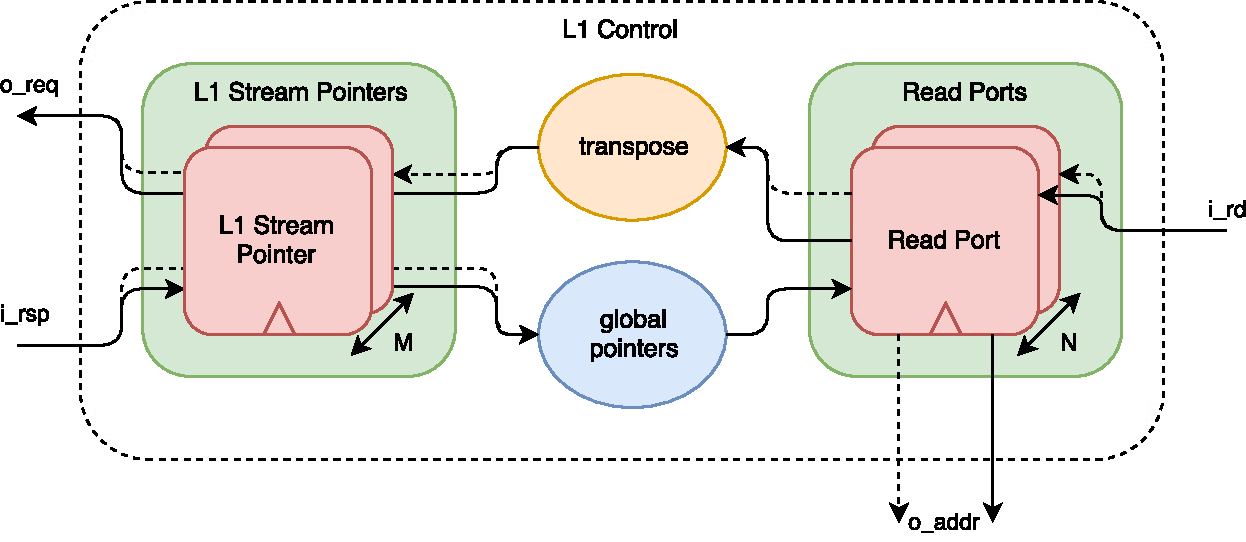
\includegraphics[width=0.70\textwidth]{5-l1-ctrl-top-b.pdf}
  \caption{Diagram of the L1 control and data path showing the essential submodules.}
  \label{fig:5-l1-ctrl-top}
\end{figure}



\subsection{L1 Stream Pointer}
\label{sec:l1-ptr}
\autoref{fig:5-l1-stream-ptr} shows the L1 stream pointer, which is a controller to keeps track of the current read pointer within the BRAM and requests new cache lines from L2 when necessary. Each stream has its own dedicated controller and all controllers are identical. Since multiple streams share a single BRAM, care must be taken in properly calculating the addresses and updating the global pointer per stream, depending on the number of read ports accessing that particular stream per cycle. In the desired configuration, that could be any number of read requests between zero and eight, the number of read ports.

\begin{figure}[H]
  \centering
  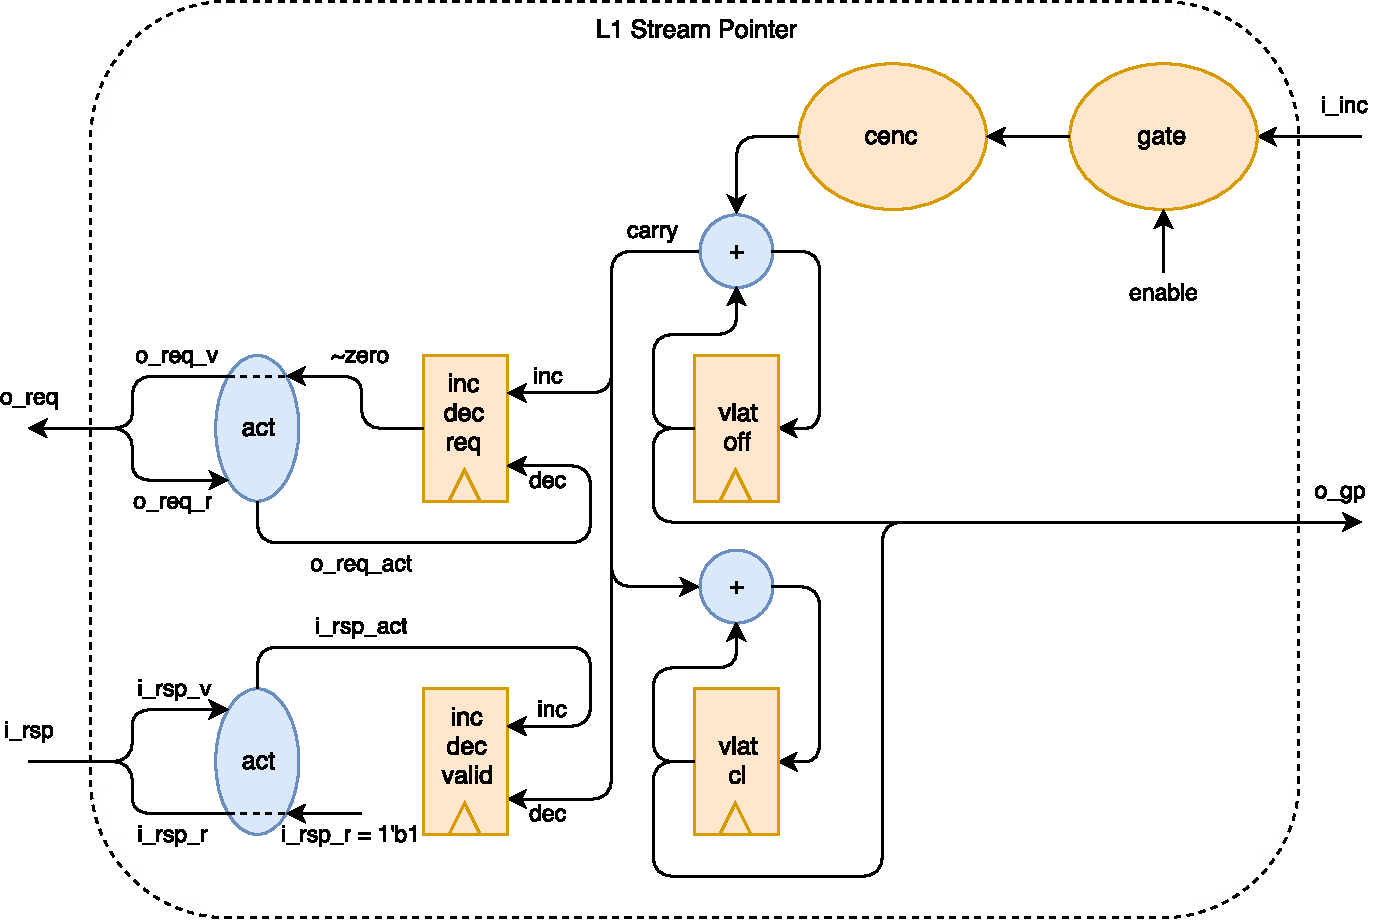
\includegraphics[width=0.70\textwidth]{5-l1-stream-ptr.pdf}
  \caption{Diagram of the L1 stream pointer module showing the essential submodules.}
  \label{fig:5-l1-stream-ptr}
\end{figure}

\subsubsection{Global Offset and Cache Line Pointer}
At the heart of each L1 stream pointer is the global stream pointer. This pointer keeps track of which address has to be read next in the BRAM to obtain the next data element. The pointer consists of two parts, one to indicate the cache line, ranging between zero and fifteen, and one to indicate the offset within the cache line, ranging between zero and seven. This global pointer is used by the read port modules to calculate the address for each AFU read request. Each cycle, all AFU read request stream identifiers are presented to the L1 stream controllers as a matrix of the number of AFU read ports times the number of streams and each stream receives a vector with the number of read ports as width. This is a one-hot encoded vector, indicating which read port (if any), made a request for this particular stream. If so, the bit is high, otherwise it is low. This vector is then fed into a count and encode module which counts the number of asserted bits. This number in turn is added to the global pointer.

\subsubsection{Valid and Request Counters}
Besides the global pointer, two counters are present which can be incremented and decremented. One counter keeps track of the number of valid cache lines in the BRAM, where each cache line consists of eight elements. This counter puts back-pressure on incoming AFU read requests when there are no valid cache lines to read. In order to minimize the size of the counter and because the cache lines are assumed to be 128B aligned and therefore the offset within each cache line starts at zero, the counter granularity is in number of cache lines. In the desired configuration, each stream has at most sixteen valid cache lines in L1. Initially the number of valid cache lines is zero. The amount is increased when L2 write responses are received which indicate that a new cache line has been read from the URAMs and written in the BRAMs. The amount is decreased when the carry bit of the offset part of the global pointer goes high. This means that the seventh element within cache line \textit{N} has been read and that the next read element will be the first element of cache line \textit{N+1}.\\
The second counter keeps track of the number of outstanding requests to the associated L2 stream controller. This means that as long as the number of valid cache lines within L1 is less than sixteen, requests have to be made to the L2 control logic to write new cache lines in the BRAM organisation. The purpose of this counter is keep the L1 buffer filled. Inversely to the valid counter decrement condition, when the carry bit is high, the request counter is incremented because a cache line has been completely read and therefore it has to be replaced with a new valid (unread) cache line. Finally, when an L2 stream request has been accepted, the request counter decrements by one.

\subsubsection{Functional Reset Behaviour}
When a functional reset occurs for this stream, it means that the corresponding L2 stream controller has been functionally reset successfully. A reason for this not to occur is for example when the respective stream still has valid data from the previous functional reset for this stream. When a functional reset of an L1 stream controller occurs, the output of the valid counter is set to zero and the output of the request counter is set to sixteen (number of cache lines per L1 stream). For the particular stream, the functional reset interface between the L1 stream controllers and the AFU is deasserted. At this point, the L1 stream controller is waiting to have at least two valid cache lines available before servicing AFU read requests. The reason is that the AFU is able to read across a cache line boundary and in order to service those, both cache lines need to be present.\\
As mentioned earlier, streams are directly mapped onto the memory organisations. During a functional reset, also a subset of the EA of the first cache line for this stream is sent from L2 to L1. The part of the global pointer which indicates the current cache line gets assigned this address as a starting value.\\
Each L2 stream controller keeps track of the current address and end address of each stream. When the end of the stream is reached, the corresponding L1 stream controller will be notified. At that point, the conditions for accepting an AFU read request change since now a read request will not only be accepted when there are two or more valid cache lines, but also when there is only one valid cache line present. After the final cache line has been fully read, the functional reset interface is asserted to indicate the end of the stream has been reached.



\subsection{Read Port Module}
\label{sec:rd-port}
\autoref{fig:5-l1-read-port} shows a high level diagram of the read port module. The purpose of a read port module is to calculate the BRAM address and update the global stream pointer based on the requested stream by the AFU. An AFU read request consists of a valid bit and the requested stream number. Since the AFU read request drives two separate control flows, both have to be synchronised. That means that no new AFU read request can be accepted until both flows have finished and are ready. In order to achieve this, the base combine module is used from the library. In order to update the L1 global stream pointer, each read port module decodes the stream identifier requested by the AFU as a one-hot signal. All decoded stream identifiers together form a matrix which is transposed and fed to the respective L1 stream controllers as discussed previously.

\begin{figure}[H]
  \centering
  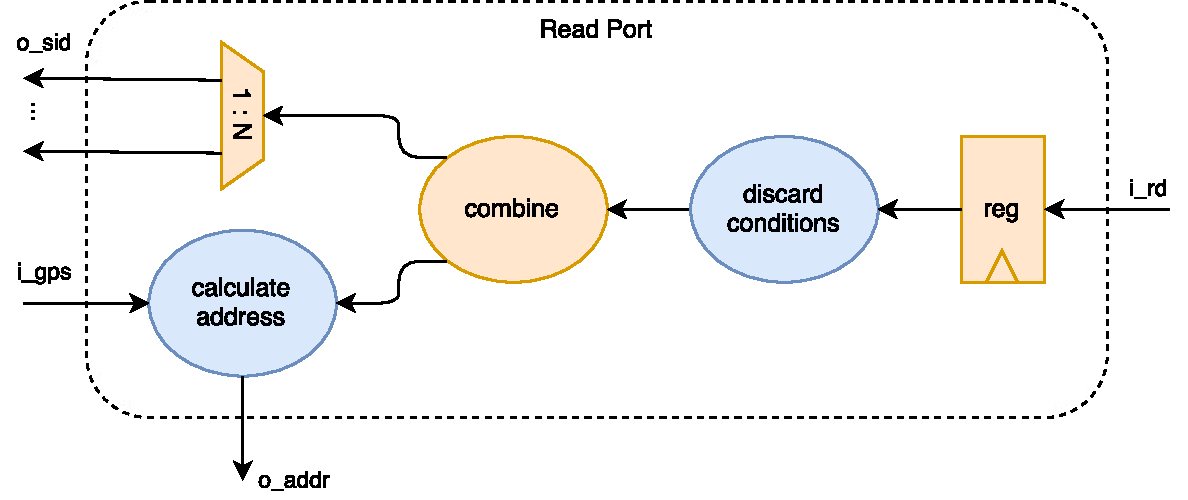
\includegraphics[width=0.70\textwidth]{5-l1-read-port.pdf}
  \caption{Diagram of a read port module showing the essential submodules.}
  \label{fig:5-l1-read-port}
\end{figure}



\subsubsection{BRAM Address Calculation}
The calculated address per read port depends on the requested stream and the requested streams of the previous read ports during that cycle. What this means is that the read ports have a predefined order, in the desired configuration ranging between zero and seven. When multiple read ports request the same stream, assuming all upstream modules are ready, read port zero will read the first unread element in the data stream, read port one the second unread element and so forth. This means that the address for read port zero equals the global stream pointer, provided by the respective L1 stream pointer module. If read port one requests the same stream, its address is equal to the global pointer plus one, since the previous read port already reads the data element at the global pointer address. In a general, this relationship can be expressed as shown in \autoref{eq:addr}.

\begin{equation}
  A(p, s) = \begin{cases}
  g(s[p])                                   & \text{if } p = 0 \\
  g(s[p]) + \sum_{n=0}^{p-1} (s[p] == s[n]) & \text{if } p > 0
  \end{cases}
  \label{eq:addr}
\end{equation}

Here \textit{A} is the BRAM address, \textit{p} is the read port number, \textit{s} is an array with the stream identifier of every read port in this cycle and \textit{g} is an array of the global pointer of each stream, provided by the L1 stream controllers. Calculating the address for any read port is basically a function of the read port number and all requested streams for that cycle. This expression consists of two parts, one statically generated as hardware, and one dynamically assigned during operation. Indexing the array of requested streams is done statically in hardware and is therefore indicated by $[]$ brackets. The global pointer array is dynamically indexed using the result of the requested stream array and is indicated by $()$ brackets. The expression also shows that, depending on the read port identifier, different logic for address calculation is generated from the same template.

\subsubsection{Preventing Deadlocks}
\label{sec:deadlocks}
With the previously described implementation, deadlocks are possible in one or multiple read port modules. In such a case, a read request for some reason can not be serviced and therefore requests for that particular read port will not make any progress. In the process, this will stall any other read requests until the deadlock has been resolved, or more common, stall for an infinite amount of time. There are three distinct scenarios where a deadlock in a read port module can occur.
\begin{itemize}
  \item{\textbf{Servicing a read request before functional reset} results in reading invalid data and should therefore be discarded.}
  \item{\textbf{Servicing a read request after a stream ended} also results in reading invalid data. When the L1 stream has ended, which also implies L2 has ended, servicing read requests should be discarded.}
  \item{\textbf{Termination of a stream mid-cycle} occurs when during a single cycle multiple read requests are made for the same stream, but after a subset of the requests (in increasing port number order), the stream ends and the successive read ports will read invalid data.}
\end{itemize}
In either case, the read request should be discarded to prevent a deadlock. This is done by testing various conditions and de-asserting the valid read signal before it reaches the \texttt{combine} cell shown in \autoref{fig:5-l1-read-port}. The reason is that when a read is discarded, the two upstream control flows are not allowed to notice the request or invalid data will be read and the global pointer will be updated while invalid data was read.\\
\autoref{fig:5-l1-read-port} also shows a \textit{discard conditions} module, which tests the deadlock conditions. While a properly designed AFU should use the provided functional reset interface to decide if a read request for a particular stream is valid, the implementation assumes a naively designed AFU. The first two scenarios can be solved by checking the output reset end signal provided by each L1 stream controller. This signal (\texttt{invalidate\_rd}) is asserted when the stream has not yet been functionally reset or when it has terminated. Therefore, if for the requested stream this signal is asserted, the read request should be discarded. A discard simply de-asserts the valid signal from the ready-valid signal pair.\\
The third scenario requires to check multiple conditions. Reading out-of-bounds only occurs when the L2 stream controller is finished and the last valid cache line in L1 is being read. If within a single cycle a read port requests the last element from the last valid cache line and a successive read port requests the same stream, the requested element is out-of-bounds since the stream has ended. If the cache line offset carry bit of the calculated address is asserted in the same cycle as the previous two conditions, the read request should be discarded.

An implication of this approach is that if the AFU makes a request and it is discarded, there is no way of knowing in the current implementation. Currently the only guarantee is that each read port operates in-order, but responses can come back to the AFU with different time offsets between read ports, depending on the amount of back-pressure on upstream modules. The current implementation provides the stream identifier as a response with the requested data element. Since streaming accesses are always in the same order, the AFU can determine the order of the response data.\\
The problem could be solved by, for example, providing the AFU with a discard signal per read port which will be asserted when this occurs. Another solution could be to associate a unique identifier (UID) with each AFU read request, which might as well be the address the BRAM was indexed with, since it will not be reused unless that index was read. The UID will be immediately returned to the AFU, after which the AFU can act accordingly.\\
However, in order to minimise wasted cycles of processing discarded read requests, the AFU could pay attention to the output reset end signal, which is asserted when the L1 stream has ended. Therefore no more valid data is present for that stream and no more requests have to be made. This solution is sufficient for the first case, but not for the second case since this output signal is not updated until after the current cycle, since a register has to be updated. For the third case, at most the number of read ports minus one reads are discarded. Another solution is to reset the AFU with the same start and end EAs as the L1 and L2 control modules. Then counters are used to keep track of the number of received responses for each stream within the AFU.





\section{BRAM Organization}
The memory organization has been discussed extensively. The idea is to have a BRAM column for each AFU read port, and each read port has access to identical data. Due to the fixed configurations of BRAM primitives and the need for four write channels, each BRAM column consists of four slices, where each slice holds one forth, or sixteen streams, which each hold sixteen cache lines per stream. The BRAM primitives are double-pumped in order to utilize them fully.

\subsection{Ready-Valid Memory Interface}
\label{sec:rvmem}
A BRAM primitive is inherently not directly compatible with the design methodology used. Memory primitives, either read or write, consist of three signals: enable, address, and data. In such a case a latch oe module is used, which is similar to a register with a so-called output enable signal, to act as a read enable input of the BRAM. This signal is triggered when the input is valid and the upstream module is ready.\\
This solution works when the operating frequencies of the control and data path are the same. When using the design methodology with back-pressure, it is important to control the enable signal of the registers within the BRAM as well or things will not work properly when there is back-pressure. For example, when using a two cycle read memory latency, two \texttt{latch\_oe} modules could be cascaded. However, since our data path is operating at twice the control frequency, a different scheme has to be used, while still supporting back-pressure. By switching to a credit-based interface, using source and sink compatible modules, back-pressure does not have to be supported in the data path but is supported by using a FIFO in the credit source module. Any additional registers within the BRAM read path can be enabled all the time, since they do not have to support back-pressure. Implementing a more sophisticated register enable signal is strictly a power optimization.

\subsection{Double-Pumped and Credit-Based BRAM}
Due to the requirement of double-pumping the BRAMs, switching to a credit-based interface is easier since it removes the requirement of controlling the pipeline registers within the BRAM in order to allow for back-pressure. This is at the cost of a six entry, 16B wide FIFO to act as the credit sink. Also multiple register stages are used in the data read path to be able to route the output signals back to the AFU. Examples are the additional pipeline register within the BRAM primitive and the FIFO within the \texttt{credit\_snk} cell.\\
\autoref{fig:5-double-pump} shows a high level diagram of the implementation of a single BRAM column using a credit-based interface. This module will be instantiated as many times as there are AFU read ports and the respective write channels are tied together.\\
The BRAM slice shown in the figure is a concatenation of eight BRAM wrapper modules to form a cache line wide memory. A BRAM wrapper module is an abstraction of the \texttt{clk2x} domain. It is basically the BRAM primitive instantiation, immediately followed by an 8:1 MUX at half the data width (8B) to select the requested element of 16B from the cache line of 128B. Then there is a free-running register at \texttt{clk2x} for the enable signal of the read pipeline register. For clarity, the write interface of each BRAM slice is not drawn, but in the desired configuration, four write channels are present.\\
The control path is shown in the upper half of the figure and operates at \texttt{clk1x}. The lower half is the data path and operates at \texttt{clk2x}. Since the \texttt{credit\_src} cell does not depend on a clock for the valid logic, an input register is added. The toggle flip flop acts as the LSB for the cache line read address. Instead of using the latch oe module to generate a read enable signal, a register is used where the output ready signal is constantly high. The reason is that the FIFO inside of the credit sink module handles received data from the BRAM. The ready-valid outputs of the \texttt{credit\_src} cell generate an act signal which is the read enable of the BRAM slice and it toggles the read address LSB flip flop. The \texttt{vlat} cell shown at the output of the BRAM acts as an alignment register to obtain the full data width again before it goes into the credit sink.

\begin{figure}[H]
  \centering
  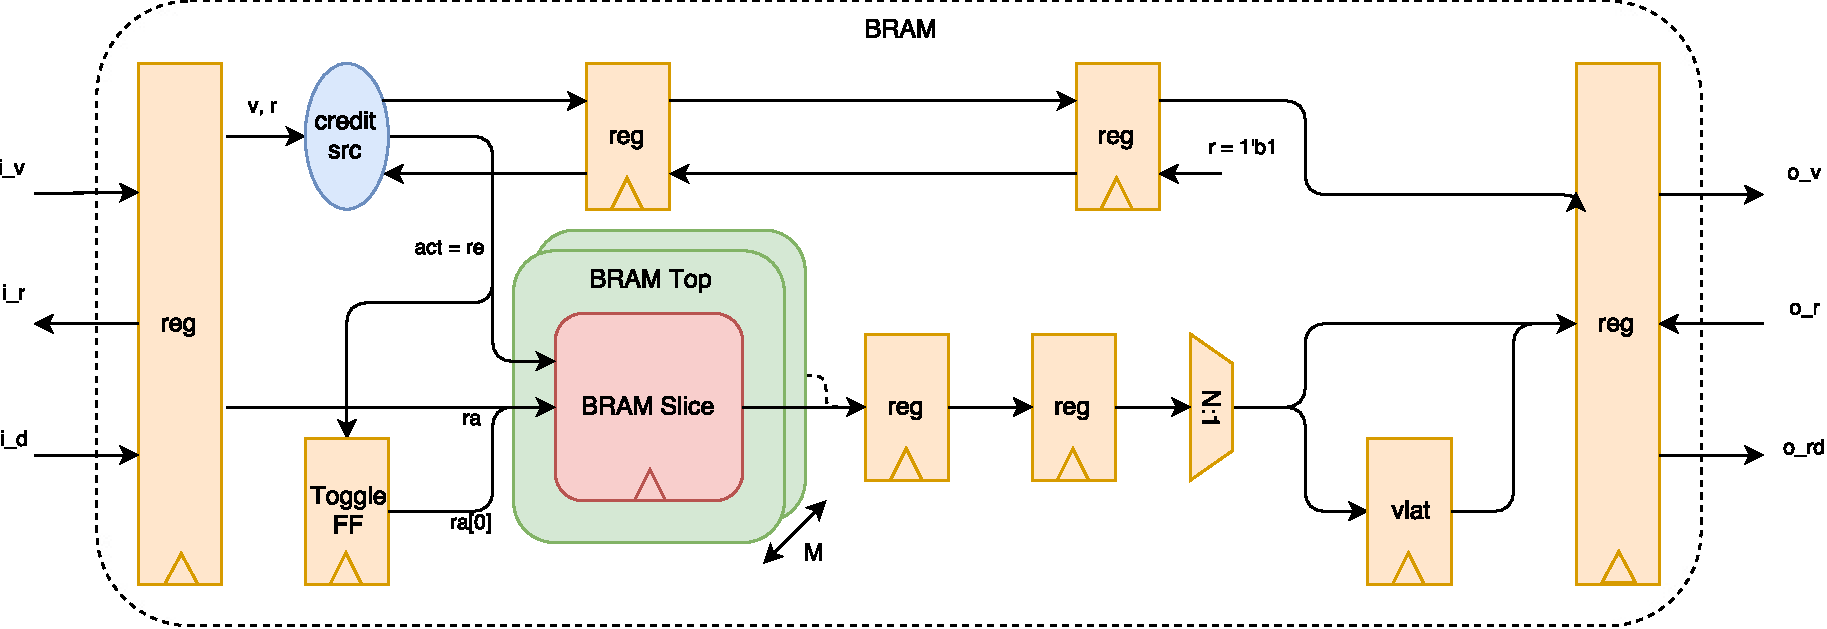
\includegraphics[width=0.75\textwidth]{5-double-pump.pdf}
  \caption{Diagram of double-pumped BRAM column using a credit-based interface.}
  \label{fig:5-double-pump}
\end{figure}

\subsection{Absence of Write Channel Back-Pressure}
Usually the ready signal is supplied by an upstream (output) or downstream (input) module, but an example of a fixed ready signal is the input response from L2 when a new cache line has been written in the BRAM organisation. This ready signal is always asserted, which means that response can always be serviced right away. The reason is that there is no back-pressure present on the write interface of the BRAMs, since the only case where back-pressure is desired is when the read and write port have a conflict. This will never occur in this implementation since a read to a specific address is only issued when that particular cache line is known to be valid, and a cache line is only written to a particular address when it is known to be invalid.





\section{L2 Control}
The second level of the design, shown in \autoref{fig:5-l2-ctrl-top}, consists of the L2 stream pointer logic, Round-Robin multiplexers and URAM organisation. The input request signal \texttt{i\_req} is connected to the L1 control output request signal \texttt{o\_req} and is as wide as there are streams. When one or multiple of these bits are asserted, a new cache line for that stream has to be fetched from the URAM organisation and written into the BRAMs.\\
However, since there are multiple L2 stream controllers within the same slice, a Round-Robin multiplexer grants read access to only one stream per slice. In the desired configuration, this is a sixteen-to-one Round-Robin multiplexer. In general, there are \textit{M} slices, each with there own output address signal \texttt{o\_addr}.\\
When a new cache line is fetched from the URAMs and written into the BRAMs, the corresponding L2 stream pointer decrements its valid counter and therefore requests a new cache line from the host. Since there is only one channel, for example OpenCAPI, to make these requests on, the same Round-Robin multiplexer modules are used to arbitrate between requests from all streams. Each slice instantiates its own Round-Robin multiplexer module after which a final Round-Robin multiplexer arbitrates between the slices.

\begin{figure}[h]
  \centering
  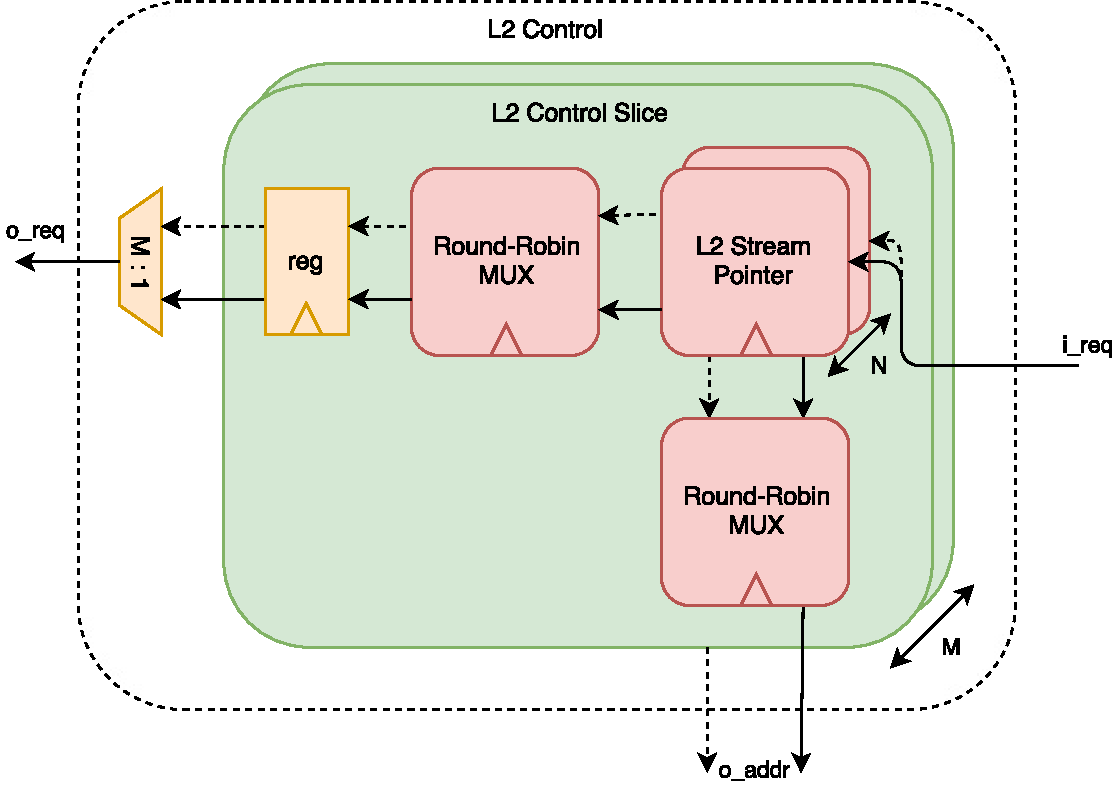
\includegraphics[width=0.60\textwidth]{5-l2-ctrl-top.pdf}
  \caption{Diagram of the L2 control and data path showing the essential submodules.}
  \label{fig:5-l2-ctrl-top}
\end{figure}



\subsection{L2 Stream Pointer}
\autoref{fig:5-l2-stream-ptr} shows the L2 stream pointer module, which is similar to the L1 stream pointer module. The input request signal \texttt{i\_req} is connected to the output request signal \texttt{o\_req} from the L1 stream pointer module. This signal is asserted when a cache line has been fully read by the AFU and indicates that the respective L2 stream pointer should fetch a new cache line from the URAMs and write it into the BRAMs.

\begin{figure}[h]
  \centering
  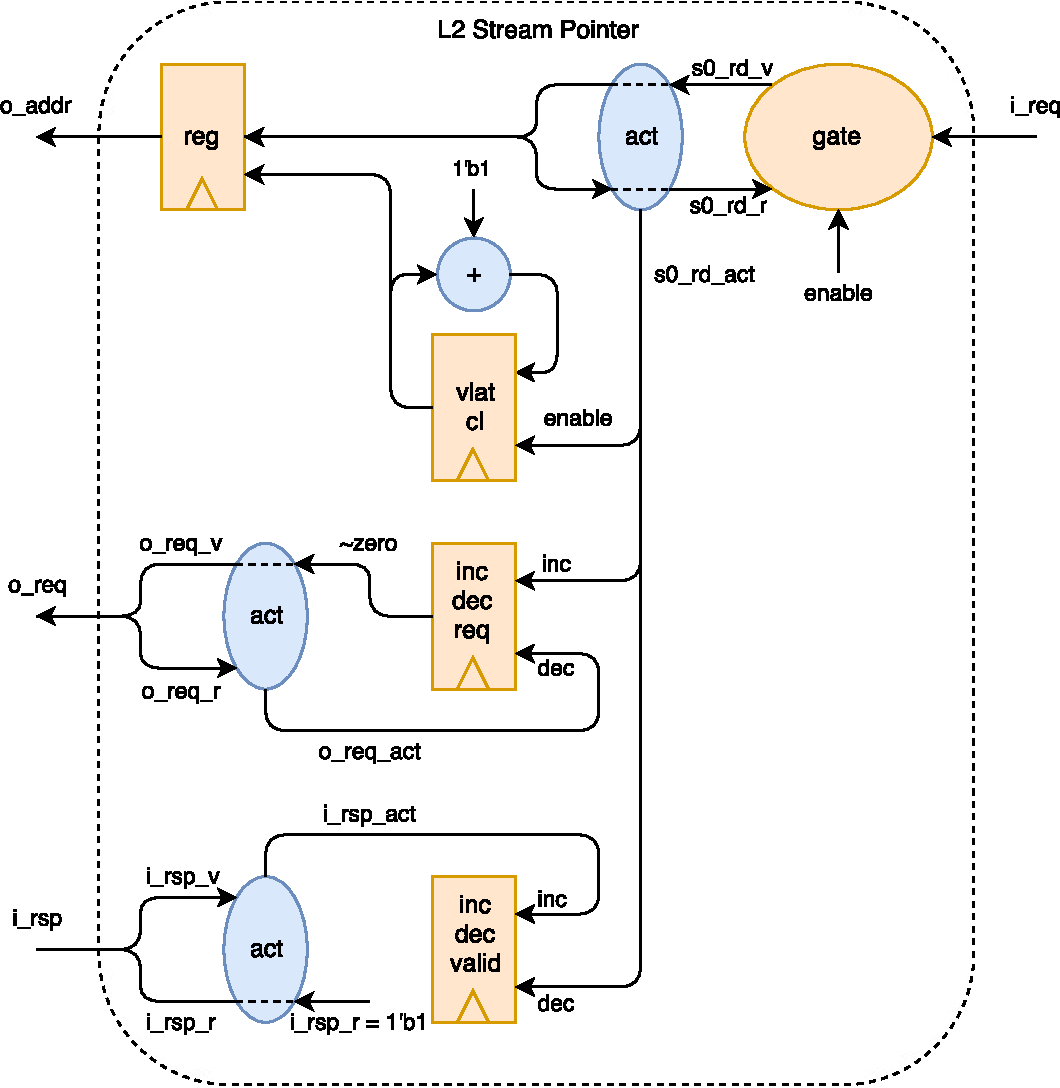
\includegraphics[width=0.70\textwidth]{5-l2-stream-ptr.pdf}
  \caption{Diagram of the L2 stream pointer showing the essential submodules.}
  \label{fig:5-l2-stream-ptr}
\end{figure}

\subsubsection{Global Cache Line Pointer}
The input request signal is first connected to a gate module, which only passes the input signals if the enable signal is asserted. In this case, the enable signal checks if there is at least one valid cache line available in the URAM for this stream. Then, the act signal \texttt{s0\_rd\_act} is generated and enables the cache line pointer, which keeps track of the current address of a particular stream. When a valid input signal occurs, the respective URAM address to be read is presented at the output signal \texttt{o\_addr}. This output signal is used to index the URAM slice.

\subsubsection{Valid and Request Counters}
Similarly to the L1 stream pointer module, there is a valid and request counter present. Instead of keeping track of sixteen cache lines per stream, as was the case for the L1 control, the L2 controllers keep track of 256 cache lines, as shown in Section \ref{sec:l2-buffer-depth}. Both counters operate in the same way as their L1 counter part, except that the act signal mentioned earlier drives the request counter increment and valid counter decrement signals. The reason is that when an input request is received, the valid counter has to be decremented since a cache line will be transferred to the L1 BRAMs. Also, the request counter is incremented since the transfer of a cache line entails an empty line in the URAMs.

\subsubsection{Functional Reset Behaviour}
On reception of a functional reset, the request first goes to a gate module, in order to assess if a functional reset is permitted. This is only the case when the respective stream has consumed all of the cache lines from the previous data stream and has no more valid cache lines in the URAM, nor outstanding requests. Both counters are used to assess these conditions.\\
If the functional reset is permitted, the request will be forwarded to the respective L1 stream controller as well and an act signal will be generated. This signal is used to initialise registers for the reset begin and end EAs respectively. The begin EA will be incremented during operation and holds the next EA to be requested from the host to fetch a new cache line. This address is sent alongside an output request from this stream. The end EA is used to determine when the stream has ended and no more cache lines have to be fetched.\\
Also the cache line pointer is reset with the direct mapped address based on the begin EA signal. This same address is sent with the response data from the URAM to index the BRAM during the write operation. The valid and request counters are reset to their initial values, thus zero valid cache lines and 256 outstanding requests. In the case that a data stream contains less than the URAM capacity per stream (less than 256 cache lines), there is logic present which decrements the valid counter by one every cycle to slowly converge to the end of a stream condition.



\subsection{Round-Robin Multiplexer}
%\todo{- Future work: weighted RR MUX to fight address translation misses. See: \url{http://www.rtlery.com/components/ppc-based-weighted-work-conserving-round-robin-arbiter}\\
%}

The Round-Robin multiplexer module consists of multiple Round-Robin multiplexers from the design library. Contrary to a traditional multiplexer, which uses an input select signal to select one out of multiple inputs, a Round-Robin multiplexer selects an input autonomously, according to a Round-Robin arbitration scheme, and produces an output select signal which indicates which of the inputs have been selected.

\subsubsection{The Need for Pipelining}
Round-Robin arbitration allows multiple requestors to share a common resource within a fixed time slot. All processes which are ready are serviced in a circular manner without the notion of priority. When a requestor has been serviced, it will go to the end of the line and will be the last to be serviced again, assuming that all requestors have a valid request.\\
For the modules used from the design library, this means that the multiplexer will first check if input \textit{N} is valid. If it is, it will be selected and during the next cycle input \textit{N+1} will be assessed, and so on. If an input is not valid, the next input will be assessed until a valid one is found, or until a full circle has been made assessing all inputs, where none were valid.\\
Due to the possibility of not a single valid input, the arbitration logic could be assessing every input. Therefore, the critical path scales with the number of inputs, or requestors. In the desired configuration, each L2 slice has to merge requests from sixteen streams to share the associated URAM (the common resource). Naively a sixteen-to-one Round-Robin multiplexer from the design library would be instantiated, but due to the number of requestors, achieving the desired operating frequency will be challenging. Therefore multiple smaller Round-Robin multiplexers are instantiated and their output is captured in a register, as shown in \autoref{fig:5-l2-rr-mux}.\\
Configuring each Round-Robin multiplexer in the top layer for four requestors results in an equally shared critical path on both sides of the register, neglecting wire delay. This results in a configuration where parameter \textit{N} equals parameter \textit{M} which equals four. Finally a second layer of a Round-Robin multiplexer is needed to merge the four outputs present after the register and present the downstream logic with a single chosen requestor. The associated data is presented at the output signal \texttt{o\_req} and the selected requestor at \texttt{o\_sel}.

\begin{figure}[H]
  \centering
  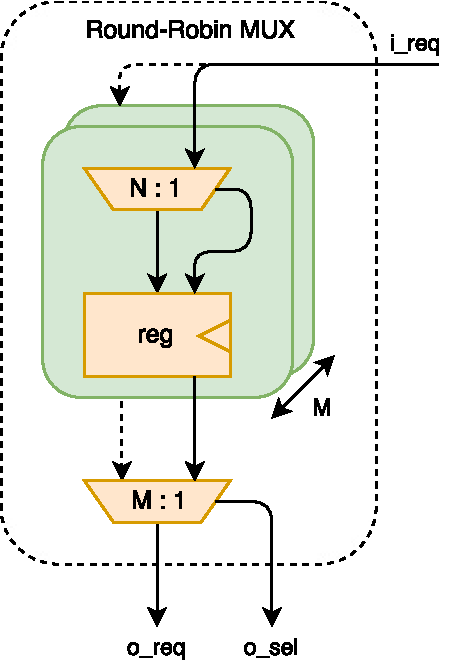
\includegraphics[width=0.35\textwidth]{5-l2-rr-mux.pdf}
  \caption{Diagram of the L2 Round-Robin multiplexer showing the essential submodules.}
  \label{fig:5-l2-rr-mux}
\end{figure}

\subsubsection{Use Cases within the L2 Control Logic}
As shown in \autoref{fig:5-l2-ctrl-top}, the Round-Robin multiplexer has two different use cases. First of all, it is used to merge the requested address from each slice of L2 stream controllers to access the associated URAM array. The data sent with a request consists of the current stream pointer, supplied by the respective L2 stream pointer module. The output select signal of the Round-Robin multiplexer is the selected stream identifier and is concatenated with the stream pointer to obtain the URAM address.\\
This module is also used for merging the host requests from all streams, shown to the left of the L2 stream pointer modules in \autoref{fig:5-l2-ctrl-top}. In the per slice use case, the data input of the Round-Robin multiplexer consists of the EA requested by each stream and the output select signal shows which stream has been chosen. When merging all slices, an additional four-to-one Round-Robin multiplexer from the design library is used, preceded by a register due to critical path considerations mentioned earlier. The input data of this final level of multiplexing is both the requested EA and the previously generated output select signal, or stream identifier. The output select signal of the final Round-Robin multiplexer indicates the selected slice and when concatenated with the previously obtained stream identifier (the output select signal of the Round-Robin multiplexer module) it represents the final chosen stream.





\section{URAM Organisation}
Contrary to the BRAM organisation, the URAM organisation has no data duplication and consists of a module called URAM Top which is generated \textit{M} times, or as often as there are write channels between L1 and L2. \autoref{fig:5-l2-uram} shows the organisation and additional submodules used.

%\todo{
%- add additional reg on control output and write output.\\
%}

\begin{figure}[H]
  \centering
  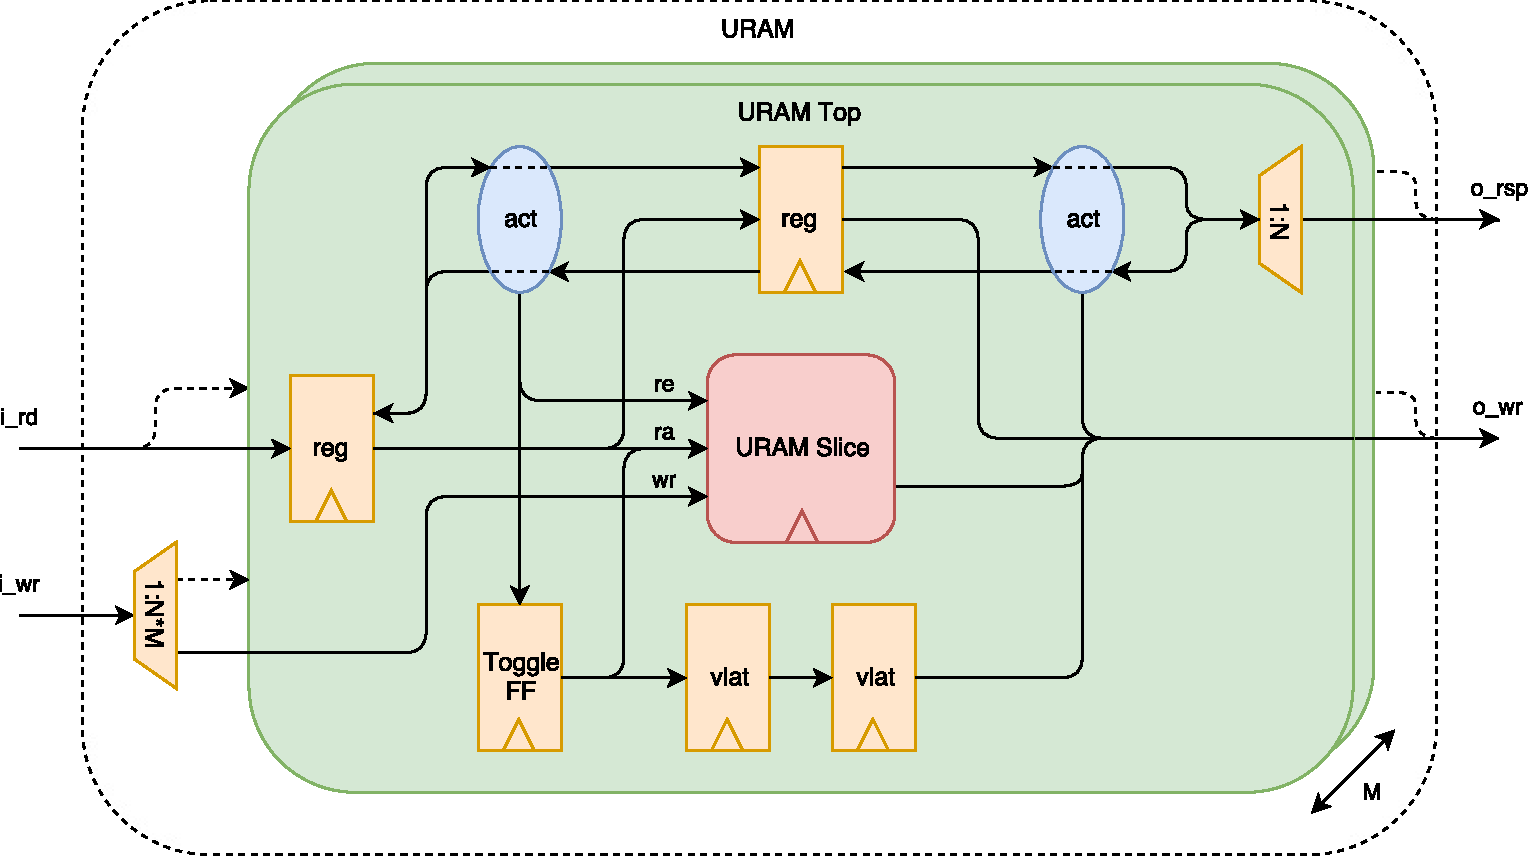
\includegraphics[width=0.80\textwidth]{5-l2-uram.pdf}
  \caption{Diagram of the URAM array for \textit{M} channels showing the essential submodules.}
  \label{fig:5-l2-uram}
\end{figure}

\subsection{URAM Slice}
A URAM Slice module consists of a concatenation of double-pumped URAM primitives. Each primitive is a 4k entry with 8 bytes per entry. By double-pumping, a 2k entry with 16 bytes per entry memory is obtained and now each entry functions as a data element. Currently the URAM primitive is configured to have a two cycle read latency, but depending on the implementation this can be changed to four cycles as well. An additional register stage is implemented to be able to route the output data from the URAM Slice to each BRAM array.

\subsection{Write Interface}
In order to write to the URAM Slice, the input write interface is present denoted by \texttt{i\_wr}. This interface is double-pumped and consists of an address and half-sized data to be written. Part of the address indicates to which channel the data should be written, which is used as the select signal of the multiplexer.

\subsection{Read Interface}
The input read interface \texttt{i\_rd} is connected to the output read interface of the L2 control module and consists of a ready-valid pair and an address (stream identifier and pointer). The interface is fed into a register after which an act signal is generated which acts as a read enable signal to the URAM Slice. It also drives the enable signal of a toggle flip-flop which operates at clk2x. Its function is to generate the least significant bit of the read address for the URAM Slice, which is concatenated with the address supplied by the input read interface. This bit is required due to the double-pumping since two addresses have to be read in a single clk1x cycle.\\
To keep the ready-valid pair synchronized with the URAM Slice, a register is used which operates at clk1x, shown above the URAM Slice in \autoref{fig:5-l2-uram}. Also the address from the input read interface is registered here since it is required to write the obtained data into the respective BRAM arrays. The earlier mentiond LSB of the address is also registered, shown below the URAM Slice, but these modules operate at clk2x.\\
Finally, an act signal is generated which represents a write enable for the output write interface \texttt{o\_wr}. The remaining signals of this interface are the address, registered in two different flows and the read data from the URAM Slice. The output write interface is directly attached to the input write interface of the BRAM arrays.\\
A response is sent to the respective L1 stream controller that a new cache line will be written into the BRAM arrays. Depending on the configuration, one URAM Top module contains \textit{N} streams, which in the desired configuration is sixteen.





%\section{Interface}

%\subsection{Request Generation}

%\subsection{Reorder Buffer}

%\todo{- reorder buffer (ROB) used in tomasulo: \url{https://en.wikipedia.org/wiki/Re-order buffer}
%}

%\todo{Some questions i asked myself during implementation of the reorder buffer and why not using a valid cache line array like in a cache.

%Comment on out of order/in order and reorder buffer versus valid cache line arrays

%if mem resources are too expensive for your design, then you might want to consider doing everything out of order instead of using a reorder buffer. if you do everything out of order you need valid arrays for every memory resource and a way to buffer read requests to memories if they cant be satisfied. that would mean that you need to converge to a cache like architecture instead of a streaming one.

%Why reorder buffer and not valid cache line array?

%reorder buffer would cost 64 streams x 2 arrays x 256 cache lines = 32K in L2.
%its easy to implement, since it fits in between the tag module and valid incdec counter.
%valid incdec then shows how many cache lines are valid in sequence from the current pointer in that stream.
%L1 doesnt need any modification since it will receive new cache lines in order from L2.

%valid array costs less in hardware;
%L1: 8 duplication x 64 streams x 16 cache lines = 8K
%L2: 4 urams x 16 streams x 256 cache lines = 16K
%Total = 24K which is less than 32K.
%However, reading from the valid arrays adds latency, but allows for out of order reading from the bram and uram. it is more difficult to implement since both l1 and l2 ctrl have to be modified. it is more like a cache structure which could be something for future work.
%However, lets look at L2 with valid cache line arrays. If you request a line from stream 0 and at the same time get a response with a line for stream 0, you run into problems. So then you would also end up with twice as many arrays to have one for req and one for rsp. then it is more expensive in hardware compared to the reorder buffer.
%}
